%%%%%%%%%%%%%%%%%%%%%%%%%%%%%%%%%%%%%%%%%%%%%%
%
%		My Thesis
%
%		EDOC Template
%		2011
%
%%%%%%%%%%%%%%%%%%%%%%%%%%%%%%%%%%%%%%%%%%%%%%


%%%%%%%%%%%%%%%%%%%%%%%%%%%%%%%%%%%%%%%%%%%%%%
%
%		Thesis Settings
%
%		EDOC Template
%		2011
%
%%%%%%%%%%%%%%%%%%%%%%%%%%%%%%%%%%%%%%%%%%%%%%
\documentclass[a4paper,12pt,fleqn,print,oneside]{book}

\usepackage[T1]{fontenc}
\usepackage[utf8]{inputenc}
\usepackage[english, vietnamese]{babel}
%\usepackage{bookman}

%%%%%%%%%%%%%%%%%%%%%%%%%%%%%%%%%%%%%%%%%%%%%%%
%% EDOC THESIS TEMPLATE: Variant 1.0 -> Latin modern, large text width&height
%%%%%%%%%%%%%%%%%%%%%%%%%%%%%%%%%%%%%%%%%%%%%%%
%\usepackage{lmodern}
%\usepackage[a4paper,top=22mm,bottom=28mm,inner=35mm,outer=25mm]{geometry}
%%%%%%%%%%%%%%%%%%%%%%%%%%%%%%%%%%%%%%%%%%%%%%%

%%%%%%%%%%%%%%%%%%%%%%%%%%%%%%%%%%%%%%%%%%%%%%
% EDOC THESIS TEMPLATE: Variant 2.0 -> Utopia, Gabarrit A (lighter pages)
%%%%%%%%%%%%%%%%%%%%%%%%%%%%%%%%%%%%%%%%%%%%%%
%\usepackage[libertine,cmintegrals,cmbraces,vvarbb]{newtxmath}
\usepackage{mathpazo}
%\usepackage{utopia} % Utopia font-typesetting including mathematical formula compatible with newer TeX-Distributions (>2010)
%\usepackage{pia} % on older systems -> use this package instead of fourier in combination with mathdesign for better looking results
%\usepackage[adobe-utopia]{mathdesign}
\setlength{\textwidth}{146.8mm} % = 210mm - 37mm - 26.2mm
\setlength{\oddsidemargin}{11.6mm} % 37mm - 1in (from hoffset)
\setlength{\evensidemargin}{0.8mm} % = 26.2mm - 1in (from hoffset)
\setlength{\topmargin}{-2.2mm} % = 0mm -1in + 23.2mm 
\setlength{\textheight}{221.9mm} % = 297mm -29.5mm -31.6mm - 14mm (12 to accomodate footline with pagenumber)
\setlength{\headheight}{14pt}
%%%%%%%%%%%%%%%%%%%%%%%%%%%%%%%%%%%%%%%%%%%%%%


\usepackage[T1]{fontenc}
\usepackage{lmodern}
%\setlength{\parindent}{0pt}

\usepackage{setspace} % increase interline spacing slightly
\setstretch{1.1}

\makeatletter
\setlength{\@fptop}{0pt}  % for aligning all floating figures/tables etc... to the top margin
\makeatother


\usepackage{graphicx,xcolor}
\graphicspath{{images/}}

%\usepackage{subfig}
\usepackage{booktabs}
\usepackage{lipsum}
\usepackage{microtype}
\usepackage{url}
\usepackage[final]{pdfpages}

\usepackage{fancyhdr}
\renewcommand{\sectionmark}[1]{\markright{\thesection\ #1}}
\pagestyle{fancy}
	\fancyhf{}
	\renewcommand{\headrulewidth}{0.4pt}
	\renewcommand{\footrulewidth}{0pt}
	\fancyhead[OR]{\bfseries \nouppercase{\rightmark}}
	\fancyhead[EL]{\bfseries \nouppercase{\leftmark}}
	\fancyfoot[EL,OR]{\thepage}
\fancypagestyle{plain}{
	\fancyhf{}
	\renewcommand{\headrulewidth}{0pt}
	\renewcommand{\footrulewidth}{0pt}
	\fancyfoot[EL,OR]{\thepage}}
\fancypagestyle{addpagenumbersforpdfimports}{
	\fancyhead{}
	\renewcommand{\headrulewidth}{0pt}
	\fancyfoot{}
	\fancyfoot[RO,LE]{\thepage}
}

\usepackage{listings}
\lstset{language=[LaTeX]Tex,tabsize=4, basicstyle=\scriptsize\ttfamily, showstringspaces=false, numbers=left, numberstyle=\tiny, numbersep=10pt, breaklines=true, breakautoindent=true, breakindent=6pt}

\usepackage{hyperref}
\hypersetup{pdfborder={0 0 0},
	colorlinks=true,
	linkcolor=black,
	citecolor=black,
	urlcolor=black}
\urlstyle{same}

\makeatletter
\def\cleardoublepage{\clearpage\if@twoside \ifodd\c@page\else
    \hbox{}
    \thispagestyle{empty}
    \newpage
    \if@twocolumn\hbox{}\newpage\fi\fi\fi}
\makeatother \clearpage{\pagestyle{plain}\cleardoublepage}


%%%%% CHAPTER HEADER %%%%
\usepackage{color}
\usepackage{tikz}
\usepackage[explicit]{titlesec}
\newcommand*\chapterlabel{}
%\renewcommand{\thechapter}{\Roman{chapter}}
\titleformat{\chapter}[display]  % type (section,chapter,etc...) to vary,  shape (eg display-type)
	{\normalfont\bfseries\Huge} % format of the chapter
	{\gdef\chapterlabel{\thechapter\ }}     % the label 
 	{0pt} % separation between label and chapter-title
 	  {\begin{tikzpicture}[remember picture,overlay]
    \node[yshift=-8cm] at (current page.north west)
      {\begin{tikzpicture}[remember picture, overlay]
        \draw[fill=black] (0,0) rectangle(35.5mm,15mm);
        \node[anchor=north east,yshift=-7.2cm,xshift=34mm,minimum height=30mm,inner sep=0mm] at (current page.north west)
        {\parbox[top][30mm][t]{15mm}{\raggedleft $\phantom{\textrm{l}}$\color{white}\chapterlabel}};  %the black l is just to get better base-line alingement
        \node[anchor=north west,yshift=-7.2cm,xshift=37mm,text width=\textwidth,minimum height=30mm,inner sep=0mm] at (current page.north west)
              {\parbox[top][30mm][t]{\textwidth}{\color{black}#1}};
       \end{tikzpicture}
      };
   \end{tikzpicture}
   \gdef\chapterlabel{}
  } % code before the title body

\titlespacing*{\chapter}{0pt}{50pt}{30pt}
\titlespacing*{\section}{0pt}{12pt}{*0}  % 13.2pt is line spacing for a text with 11pt font size
\titlespacing*{\subsection}{0pt}{12pt}{*0}
\titlespacing*{\subsubsection}{0pt}{12pt}{*0}

\newcounter{myparts}
\newcommand*\partlabel{}
\titleformat{\part}[display]  % type (section,chapter,etc...) to vary,  shape (eg display-type)
	{\normalfont\bfseries\Huge} % format of the part
	{\gdef\partlabel{\thepart\ }}     % the label 
 	{0pt} % separation between label and part-title
 	  {\setlength{\unitlength}{20mm}
	  \addtocounter{myparts}{1}
	  \begin{tikzpicture}[remember picture,overlay]
    \node[anchor=north west,xshift=-65mm,yshift=-6.9cm-\value{myparts}*20mm] at (current page.north east) % for unknown reasons: 3mm missing -> 65 instead of 62
      {\begin{tikzpicture}[remember picture, overlay]
        \draw[fill=black] (0,0) rectangle(62mm,20mm);   % -\value{myparts}\unitlength
        \node[anchor=north west,yshift=-6.1cm-\value{myparts}*20mm,xshift=-60.5mm,minimum height=30mm,inner sep=0mm] at (current page.north east)
        {\parbox[top][30mm][t]{55mm}{\raggedright \color{white}Part \partlabel $\phantom{\textrm{l}}$}};  %the phantom l is just to get better base-line alingement
        \node[anchor=north east,yshift=-6.1cm-\value{myparts}*20mm,xshift=-63.5mm,text width=\textwidth,minimum height=30mm,inner sep=0mm] at (current page.north east)
              {\parbox[top][30mm][t]{\textwidth}{\raggedleft \color{black}#1}};
       \end{tikzpicture}
      };
   \end{tikzpicture}
   \gdef\partlabel{}
  } % code before the title body
 
 
\usepackage{lastpage}
 
%\fancyhead[R]{
%	\begin{tabular}{l}
%		\tiny \bf \\
%		\tiny \bf 
%	\end{tabular}  }

%\fancyfoot{} % clear all footer fields
%\fancyfoot[R]{\ttfamily {\thepage}}
%\fancyfoot[L]{\scriptsize \ttfamily LUẬN VĂN TỐT NGHIỆP - Niên khóa 2014-2018}
%\fancyfoot[R]{\scriptsize \ttfamily Trang {\thepage}/\pageref{LastPage}}
%\renewcommand{\headrulewidth}{0.3pt}
%\renewcommand{\footrulewidth}{0.3pt}

\usepackage{amsmath}
% Fix the problem with delimiter size caused by fourier and amsmath packages.
\makeatletter
\def\resetMathstrut@{%
  \setbox\z@\hbox{%
    \mathchardef\@tempa\mathcode`\(\relax
      \def\@tempb##1"##2##3{\the\textfont"##3\char"}%
      \expandafter\@tempb\meaning\@tempa \relax
  }%
  \ht\Mathstrutbox@1.2\ht\z@ \dp\Mathstrutbox@1.2\dp\z@
}
\makeatother


%%%%%%%%%%%%%%%%%%%%%%%%%%%%%%%%%%%%%%%%%%%%%%
%
%		Thesis Settings
%		Custom settings
%
%		2011
%
%%%%%%%%%%%%%%%%%%%%%%%%%%%%%%%%%%%%%%%%%%%%%%

%
%   Use this file for your own custom packages, command-definitions, etc...
%


% the following lines are for creating a simplified TO-DO box. However since boites is not per default installed with all latex-distributions, we have removed this example again
% if you want to use it and do not have "boites" installed, you can get it from here: http://www.ctan.org/tex-archive/macros/latex/contrib/boites
%
%\usepackage{boites,boites_exemples}
%\newcommand{\todolist}[1]{\begin{boiteepaisseavecuntitre}{TO DO in this chapter} #1 \end{boiteepaisseavecuntitre}}  % creates a little box
% %\newcommand{\todolist}[1]{}  % to be used when to do is not to be printed
\usepackage[numbers]{natbib}
\bibliographystyle{IEEEtranN}
\usepackage[noabbrev, nameinlink]{cleveref}
\usepackage{pdfpages}
\usepackage{enumitem}
\usepackage{textcomp}
\usepackage{pifont}
\usepackage{tabto}
\usepackage{amssymb}
\usepackage{hyperref}
\usepackage{booktabs}
\usepackage{graphicx}
\usepackage{array}
\usepackage{pdflscape}
%\usepackage{subcaption}
\usepackage{subfig}
\usepackage{forest}

\makeatletter
\renewcommand*\l@figure{\@dottedtocline{1}{1em}{3.2em}}
\makeatother
  % place your custom packages, etc... in this file!
%\input{thesis-info.tex}

%%%%%%%%%%%%%%%%%%%%%%%%%%%%%%%%%%%%%%%%%%%%%%
%%%%% HEAD: Book-Begin
%%%%%%%%%%%%%%%%%%%%%%%%%%%%%%%%%%%%%%%%%%%%%%
\begin{document}
\frontmatter
%\begin{titlepage}
%\begin{center}
%%\large
%\sffamily
%
%
%\null\vspace{2cm}
%{\huge A survey of various data dissemination schemes for Vehicular Ad-hoc NETwork} \\[24pt] 
%\textcolor{gray}{\small{THIS IS A TEMPORARY TITLE PAGE \\ It will be replaced for the final print by a version \\ provided by the service academique.}}
%    
%\vfill
%
%\begin{tabular} {cc}
%\parbox{0.3\textwidth}{\includegraphics[width=4cm]{images/epfl}}
%&
%\parbox{0.7\textwidth}{%
%	Thèse n. 1234 2011\\
%	présenté le 12 Mars 2011\\
%	à la Faculté des Sciences de Base\\
%	laboratoire SuperScience\\
%	programme doctoral en SuperScience\\
%%
%%	ÉCOLE POLYTECHNIQUE FÉDÉRALE DE LAUSANNE\\
%	École Polytechnique Fédérale de Lausanne\\[6pt]
%	pour l'obtention du grade de Docteur ès Sciences\\
%	par\\ [4pt]
%	\null \hspace{3em} Paolino Paperino\\[9pt]
%%
%\small
%acceptée sur proposition du jury:\\[4pt]
%%
%    Prof Name Surname, président du jury\\
%    Prof Name Surname, directeur de thèse\\
%    Prof Name Surname, rapporteur\\
%    Prof Name Surname, rapporteur\\
%    Prof Name Surname, rapporteur\\[12pt]
%%
%Lausanne, EPFL, 2011}
%\end{tabular}
%\end{center}
%\vspace{2cm}
%\end{titlepage}

\begin{titlepage}
	%
\includepdf{head/cover.pdf}
\thispagestyle{empty}
\begin{center}
	\begin{large}
		\textbf{Đại học Quốc gia Thành phố Hồ Chí Minh}
	\end{large} \\
	\begin{large}
		\textbf{Trường Đại học Bách Khoa}
	\end{large} \\
	\begin{large}
		\textbf{Khoa Khoa học và Kỹ thuật Máy tính}
	\end{large} \\
	\textbf{--------------------  *  ---------------------}\\[1.2cm]
	
	\begin{center}
		
\includegraphics[scale=0.2]{images/logo.png}\\[1.0cm]
	\end{center}
	
	{\fontsize{23pt}{1}\selectfont \textbf{Đề Cương Luận Văn}}\\[1.5cm]
	
	{\fontsize{24pt}{1}\selectfont \textbf{Đề tài:} Hiện thực mô hình điều khiển tự động quadcopter theo cơ chế bầy đàn}\\[1.75cm]
\end{center}

\hspace{2cm} Hội đồng \hspace{72pt} :  \hspace{5pt} \textbf{\parbox[t]{10cm}{
		Kỹ Thuật Máy Tính
}} 

\hspace{2cm} Giáo viên hướng dẫn \hspace{14pt} :  \hspace{4pt} \textbf{\parbox[t]{8cm}{
		TS. Phạm Hoàng Anh
}} 

\hspace{2cm} Giáo viên phản biện \hspace{18pt} :  \hspace{4pt} \textbf{\parbox[t]{8cm}{
		ThS. Võ Tấn Phương
}} \\


\hspace{2cm} Nhóm sinh viên thực hiện : \hspace{4pt}
\textbf{\parbox[t]{20cm}{
		Trần Lê Minh \hspace{69pt} - 1412319\\
		Lê Huy Cường \hspace{64pt} - 1410432\\
		Nguyễn Hoàng Thương \hspace{13pt} - 1513396\\
}}


\vspace{1.5cm}
%	\vspace{1.75cm}
\begin{center}
	%{\fontsize{20pt}{1} TP Hồ Chí Minh}\\
	{\fontsize{20pt}{1} Ngày 30 tháng 10 năm 2018}
\end{center}

\end{titlepage}




\cleardoublepage
\thispagestyle{empty}


\vspace*{3cm}

\begin{raggedleft}
    	I think, therefore I am;\\
     --- René Descartes\\
\end{raggedleft}

\vspace{4cm}




\setcounter{page}{0}
\chapter*{Lời cam đoan}
\markboth{Lời cam đoan}{Lời cam đoan}
\addcontentsline{toc}{chapter}{Lời cam đoan}
\vspace{1.0cm}
Nhóm cam đoan mọi điều được ghi trong báo cáo, cũng như mã nguồn là do nhóm tự thực hiện - trừ các kiến thức tham khảo có trích dẫn cũng như mã nguồn mẫu do chính nhà sản xuất cung cấp, hoàn toàn không sao chép từ bất cứ nguồn tài liệu hay công trình nghiên cứu nào khác. Nếu lời cam đoan trái với sự thật, nhóm xin chịu mọi trách nhiệm trước Khoa và Nhà trường.
\begin{flushright}
Nhóm sinh viên thực hiện đề tài 
\end{flushright}


\bigskip
 
%\noindent\textit{Lausanne, 12 Mars 2011}
%\hfill D.~K.

\chapter*{Lời cảm ơn}
\markboth{Lời cảm ơn}{Lời cảm ơn}
\addcontentsline{toc}{chapter}{Lời cảm ơn}
\onehalfspacing
\vspace{1.0cm}
Sau bốn năm theo học tại khoa Khoa học Kĩ thuật Máy tính trường Đại học Bách khoa TP. Hồ Chí Minh, em đã được áp dụng tất cả những kiến thức đã học để thực hiện luận văn tốt nghiệp, đề tài cuối cùng mang tính quyết định kết quả học tập và quá trình tốt nghiệp.\\

Em xin chân thành cảm ơn quý thầy cô trong Khoa đã mang đến những kiến thức bổ ích trong suốt quãng đời sinh viên, đặc biệt là thầy Phạm Hoàng Anh đã giúp đỡ em trong quá trình thực hiện cũng như quá trình hoàn thiện luận văn. Em cũng gửi lời cảm ơn đến một số bạn bè trong Khoa đã hỗ trợ giúp em tiết kiệm được thời gian tìm hiểu đề tài. \\

Em đã cố gắng hết sức để tránh các sai sót, nhưng nếu có phát hiện thì mong quý thầy cô góp ý để em càng hoàn thiện đề tài hơn. Cuối cùng em xin gửi lời chúc sức khỏe và cảm ơn chân thành nhất.
\begin{flushright}
 Nhóm sinh viên thực hiện đề tài 
\end{flushright}

\bigskip
 
%\noindent\textit{Lausanne, 12 Mars 2011}
%\hfill D.~K.

%\input{head/achievement}
% English abstract
\cleardoublepage
\chapter*{Tóm tắt}
%\markboth{Abstract}{Abstract}
\addcontentsline{toc}{chapter}{Tóm tắt} % adds an entry to the table of contents
\vspace{1.0cm}
Phương tiện bay không người lái (Unmanned Aerial Vehicles) gần đây đã trở nên phổ biến trong nhiều lĩnh vực như do thám, truyền hình, phim ảnh, giao hàng, ... Ngoài các cảm biến tinh vi  cho những lĩnh vực đó, các UAV còn có thể được trang bị bộ giao tiếp, giúp chúng có thể giao tiếp, chia sẻ thông tin với nhau nhằm thực hiện một công việc cụ thể nào đó cần sự phối hợp giữa nhiều UAV. Trong đề tài này, nhóm sẽ thảo luận về cơ chế bay của một UAV, mô hình giao tiếp giữa các UAV và sự giao tiếp giữa UAV và máy chủ. Để chứng minh độ hiệu quả của mô hình, nhóm sẽ hiện thực các UAV bay theo cơ chế bầy đàn để thực hiện một nhiệm vụ cụ thể.
%Gần đây, khái niệm Cách mạng Công nghiệp 4.0 được nhắc đến nhiều trên truyền thông và mạng xã hội. Cùng với đó là những hứa hẹn về cuộc đổi đời của các doanh nghiệp tại Việt Nam nếu đón được làn sóng này. Cách mạng Công nghiệp 4.0 sẽ diễn ra trên 3 lĩnh vực chính gồm Công nghệ sinh học, Kỹ thuật số và Vật lý. Những yếu tố cốt lõi của Kỹ thuật số sẽ là: Trí tuệ nhân tạo (AI), Vạn vật kết nối - Internet of Things (IoT) và dữ liệu lớn (Big Data)\cite{cmcn}. Trong đó IoT sẽ đảm nhiệm việc kết nối, thu nhập thông tin từ các thiết bị và vật dụng tạo nên Big Data, còn AI sẽ đảm nhiệm việc xử lý chúng.\\

%Hiện nay các doanh nghiệp tham gia phát triển các hệ thống IoT sử dụng rất nhiều chuẩn kết nối khác nhau, có những chuẩn quen thuộc với đa số mọi người như WiFi, Ethernet, Bluetooth; cũng có những chuẩn thuộc dạng \lq\lq{}chuyên ngành\rq\rq{} như ZigBee, LoRa, Xbee, RFID. Mỗi chuẩn đều có những ưu nhược điểm riêng và phù hợp với các ứng dụng cụ thể.\\

%Trong đề tài này, nhóm sẽ thảo luận về giao thức Bluetooth Mesh, một giao thức mạng được phát triển dựa trên chuẩn giao tiếp Bluetooth. Bluetooh Mesh là một chuẩn ra đời sau, khá mới so với những chuẩn khác nên khả năng chiếm giữ thị trường còn hạn chế. Tuy nhiên với những ưu điểm đầy hứa hẹn của mình, Bluetooh Mesh sẽ nhanh chóng thay đổi bộ mặt của lĩnh vực IoT.\\

%Ngoài việc tổng hợp một số nghiên cứu của nhóm về nguyên lý hoạt động của Bluetooh Mesh để làm tài liệu tham khảo cho các khóa sau, nhóm còn tiến hành thử nghiệm hiện thực một ứng dụng đơn giản để chứng minh tiềm năng của Bluetooh Mesh. Ứng dụng bao gồm việc thu thập dữ liệu và cập nhật lên cloud thông qua mạng GPRS.


\vskip0.5cm
%put your text here


%\endgroup			
%\vfill


\tableofcontents
\pdfbookmark{\contentsname}{Mục lục}
\cleardoublepage
\phantomsection
\addcontentsline{toc}{chapter}{Mục Lục Hình} % 
%\addcontentsline{toc}{chapter}{Danh Sách Bảng} %
%adds an entry to the table of contents
\listoffigures
\cleardoublepage
\phantomsection
%\addcontentsline{toc}{chapter}{List of tables} % adds an entry to the table of contents
%\listoftables
%\cleardoublepage
%\phantomsection
\newcommand{\abbrlabel}[1]{\makebox[3cm][l]{\textbf{#1}\ \dotfill}}
\newenvironment{abbreviations}{\begin{list}{}{\renewcommand{\makelabel}{\abbrlabel}}}{\end{list}}

\chapter*{Thuật ngữ \& từ viết tắt}
\thispagestyle{empty}
\pagestyle{empty}
\addcontentsline{toc}{chapter}{Thuật ngữ \& từ viết tắt}
\vspace{1.0cm}
\begin{abbreviations}
	\item[AES] Advanced Encryption Standard 
	\item[BLE] Bluetooth Ligh Energy
	\item[BR/EDR] Basic Rate/Enhanced Data Rate 
	\item[CBC-MAC] Cipher Block Chaining Message Authentication Code
	\item[CCM] Counter with CBC-MAC
	\item[Cloud] Trong phạm vi đề tài, dùng để chỉ nơi lưu trữ dữ liệu trên internet
	\item[CMAC] Cipher-based Message Authentication Code
	\item[ECDH] Elliptic-curve Diffie–Hellman
	\item[GPRS] General Packet Radio Service
	\item[GSM] Global System for Mobile Communications
	\item[GUI] Graphical User Interface
	\item[IPv4] Internet Protocol version 4
	\item[IPv6] Internet Protocol version 6
	\item[LPN]  Low power node
	\item[Mesh] Mạng mesh là mạng mà các phần tử đều có kết nối với nhau
	\item[MITM] Man-in-the-midle: Chen giữa một kết nối nhằm mục đích xấu
	\item[Node] Node là một phần tử trong mạng mesh
	\item[OOB] Out-of-band
	\item[P2P] Peer-to-peer
	\item[TTL] Time To Live
	\item[Sleep] Trạng thái ngủ giúp tiết kiệm năng lượng
\end{abbreviations}
% your list of symbols here, if needed.


% space before each new paragraph according to the template guidelines.
%(needs to be after titlepage and frontmatter to keep the table of contents lists short)
\setlength{\parskip}{1em}


%%%%%%%%%%%%%%%%%%%%%%%%%%%%%%%%%%%%%%%%%%%%%%
%%%%% MAIN: The chapters of the thesis
%%%%%%%%%%%%%%%%%%%%%%%%%%%%%%%%%%%%%%%%%%%%%%
\mainmatter
\chapter{Giới thiệu đề tài}
\pagestyle{fancy}
Từ lúc bắt đầu có khái niệm IoT cho đến nay, đã có rất nhiều ứng dụng trong những lĩnh vực khác nhau, mang lại hiệu quả và độ chính xác cao hơn hẳn so với sức người, giảm chi phí cho sản xuất, bảo vệ môi trường,... Do đó, IoT được dự báo là công nghệ của tương lai, đóng vai trò quan trọng trong \lq\lq{}Cách mạng công nghiệp 4.0\rq\rq{}.\\

Hình dưới đây mô tả một hệ thống IoT tiêu chuẩn: các thiết bị và cảm biến trong nhóm Things sẽ kết nối, giao tiếp với nhau thông qua một mạng nội bộ, một số ứng dụng chỉ cần nhóm này là đủ nếu không có nhu cầu trao đổi dữ liệu với cloud. Gateway sẽ đảm nhiệm vai trò kết nối giữa hai loại mạng khác nhau, chẳng hạn như mạng nội bộ với cloud, mạng WiFi với ZigBee hay như trong đề tài này là mạng Bluetooth Mesh với GPRS. Sau cùng là cloud với vai trò lưu trữ dữ liệu cũng như phân tích nó, cloud còn đảm nhiệm giao tiếp với một số thiết bị có giao diện người dùng như máy tính, điện thoại,...

    \begin{figure}[h!]
    	\begin{center}
    		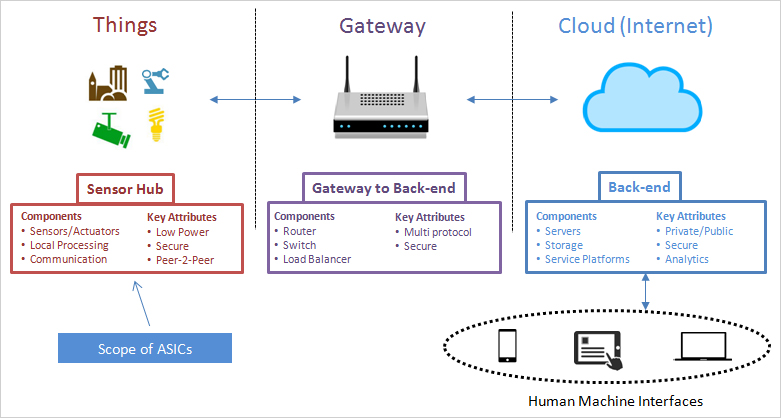
\includegraphics[scale=0.5]{images/internet-of-things-bone.jpg}
    		\caption{Một hệ thống IoT tiêu chuẩn}
    	\end{center}
    \end{figure}

Nhóm Things có thể bao gồm rất nhiều thiết bị, chẳng hạn như một hội trường cỡ vừa đã có hàng trăm bóng đèn, hàng trăm cái ghế. Do đó việc sử dụng kiểu kết nối hình sao, vòng, P2P hay cây đều có những bất lợi cũng như khó mở rộng, kết nối mesh dễ dàng đánh bại những kiểu kết nối khác trong cuộc đua này.\\

Cho đến nay đã có rất nhiều giải pháp mạng mesh không dây (wireless) sử dụng nhiều loại công nghệ khác nhau. Mục tiêu ban đầu của những giải pháp này là ứng dụng trong quân sự, sau đó là công nghiệp và cuối cùng là nhà thông minh. Lý do chính dẫn đến thất bại của WiFi và ZigBee trong việc hiện thực mạng mesh chính là thiếu khả năng liên kết giữa các nhà sản xuất, Bluetooth Mesh sẽ thay đổi điều đó\cite{meshadvan}.\\

Nhằm tìm hiểu tiềm năng trong tương lai của Bluetooth Mesh, nhóm đã thực hiện đề tài này và tổng hợp những điểm quan trọng của giao thức này trong báo cáo, làm cơ sở tham khảo cho những ai quan tâm và có ý định phát triển ứng dụng trên nền Bluetooth Mesh.\\

Báo cáo sẽ được trình bày theo thứ tự như sau:
    \begin{itemize}
        \item Chương đầu tiên sẽ giới thiệu sơ lược về đề tài và giao thức Bluetooth Mesh, liệt kê những nhiệm vụ cần đạt cũng như sơ đồ khối và cách thức hoạt động của ứng dụng thử nghiệm.
        \item Chương tiếp theo sẽ tập trung vào những gì nhóm nghiên cứu được về giao thức Bluetooth Mesh, điểm qua lịch sử, kiến trúc, nguyên lý hoạt động và cách thức quản lý các phần tử trong mạng.
        \item Chương 3 là danh sách những công cụ cả về phần cứng và phần mềm mà nhóm dùng để hiện thực ứng dụng thử nghiệm, có bao gồm mô hình thiết kế của ứng dụng.
        \item Chương 4 ghi lại quá trình hiện thực ứng dụng dựa trên công cụ của nhà sản xuất và tùy chỉnh một số mã nguồn mẫu, hiện thực thư viện giao tiếp với module GSM.
        \item Chương 5 là các kịch bản nhóm dựng lên để thử nghiệm ứng dụng, bao gồm thử nghiệm khoảng cách tối đa giữa 2 thiết bị trong mạng, giao tiếp trong mạng và hoạt động của node gateway.
        \item Chương 6 là chương kết luận, bao gồm việc đánh giá và đưa ra gợi ý cho những ứng dụng trong thực tế.
        \item Cuối cùng là tài liệu tham khảo và một số phụ lục: các model chuẩn, flowchart quá trình remote provisioning, hướng dẫn sơ lược cách sử dụng các chương trình nhóm dùng để hiện thực ứng dụng.
    \end{itemize}

    \section{Nhiệm vụ cần đạt}
    \begin{itemize}
        \item Tìm hiểu lý thuyết về Bluetooth Mesh, nguyên lý hoạt động, ưu nhược điểm,... Mục tiêu này đã hoàn thành bước đầu trong giai đoạn Đề lương luận văn. Giai đoạn luận văn sẽ nghiên cứu sâu hơn và cụ thể hơn các lý thuyết đã được trình bày ở giai đoạn Đề cương.
        \item Sử dụng các công cụ hiện có, hiện thực ứng dụng có khả năng giao tiếp giữa các thiết bị cuối - đảm nhiệm nhiệm vụ thu nhập dữ liệu và điều khiển thiết bị - và thiết bị gateway - đảm nhiệm việc giao tiếp với cloud.
        \item Đề ra các phương án áp dụng Bluetooh Mesh vào các ứng dụng thực tế, cũng như các hướng phát triển trong tương lai.
        \item Xây dựng kịch bản để thử nghiệm, chứng minh ưu điểm của Bluetooth Mesh so với các chuẩn giao tiếp khác.
    \end{itemize}
    \newpage
    \section{Sơ đồ khối}

    \begin{figure}[h!]
    	\begin{center}
    		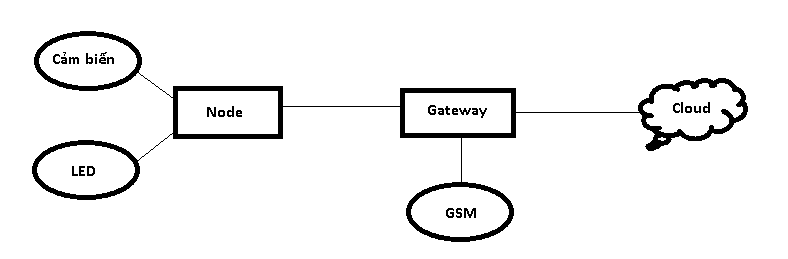
\includegraphics[scale=0.8]{images/block-diagram.png}
    		\caption{Sơ đồ khối của ứng dụng}
    	\end{center}
    \end{figure}

    \section{Hoạt động}
        \begin{itemize}
            \item Trước tiên cần tiến hành bước khởi tạo: cho phép các node cảm biến tham gia vào mạng.
            \item Ấn nút trên node gateway để kích hoạt/tắt chức năng giám sát của hệ thống. Khi trong chế độ giám sát, sau mỗi chu kỳ nhất định, node gateway sẽ gửi yêu cầu lần lượt tới toàn bộ các node cảm biến có trong mạng - quá trình này cũng cho phép kiểm tra sự tồn tại của các node trong mạng - sau đó gửi toàn bộ dữ liệu lên server. Chức năng này thể hiện hướng dữ liệu từ node cảm biến đến node gateway.
            \item Ấn một nút khác cũng trên node gateway để điều khiển LED trên tất cả các node cảm biến, chức năng này giúp cho việc kiểm thử dễ dàng hơn. Chức năng này thể hiện hướng dữ liệu từ node gateway đến node cảm biến.
        \end{itemize}


\chapter{Cơ sở lý thuyết} \label{chap:theory}
    \section{Bluetooth Mesh}
    	\subsection{Bluetooth trước Bluetooth Mesh}
Trước khi Bluetooth Mesh ra đời, Bluetooth đã phát triển đến phiên bản 5.0, trong đó có thể chia làm hai giai đoạn (hay hai sứ mạng) bao gồm Bluetooth Basic Rate/Enhanced Data Rate (BR/EDR) và Bluetooth Low Energy (LE). BR/EDR mang lại thế hệ thiết bị không dây mới như tai nghe, chuột, bàn phím không dây,... trong khi đó BLE mang lại các thiết bị chạy pin như đồng hồ thông mình, các thiết bị thể thao, định vị,... Cả hai có thể tồn tại trong cùng một thiết bị nhưng không giao tiếp với nhau.\\

Trong khi BR/EDR chỉ hỗ trợ kết nối 1:1, dễ dàng nhận thấy điều này qua việc một bàn phím không dây không thể dùng cho hai máy tính cùng lúc, hoặc một điện thoại không thể "bắn bluetooth" cho nhiều điện thoại cùng lúc; thì BLE hỗ trợ thêm kết nối 1:nhiều bằng cách thức broadcast, chúng ta có thể tìm thấy kết nối này trong các ứng dụng Bluetooth beacons.
\newpage
       \begin{figure}[h!]
	        	\begin{center}
	        		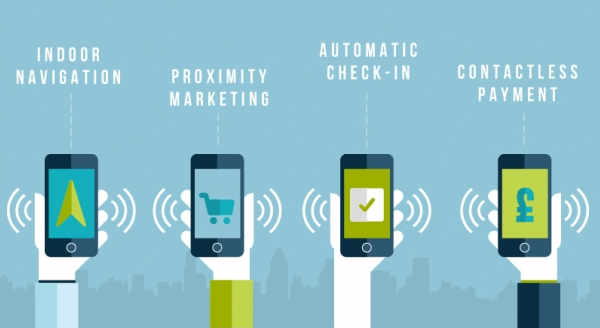
\includegraphics[scale=0.8]{images/retail.png}
	        		\caption{Các ứng dụng sử dụng Bluetooth beacons}
	        	\end{center}
        \end{figure}
        
\textbf{\textit{Vậy Bluetooth Mesh có thể mang lại những tiềm năng gì?}}
    	\subsection{Bluetooth Mesh ra đời}
Bluetooth Mesh được tổ chức SIG đưa ra các giao thức (protocol) chung vào tháng 7 năm 2017\cite{meshborn} và chia sẻ nhiều đặc điểm chung với BLE. Về cơ bản, Bluetooth Mesh sử dụng cấu trúc mạng của BLE nên các thiết bị sử dụng mạng BLE có thể tham gia mạng mesh, cấu hình của các gói tin (package) và phương thức quảng bá (advertisement) của cả 2 giống nhau. Tuy nhiên vẫn có những điểm khác nhau giữa lớp Host của cả 2 mạng. Do đó, Bluetooth là một giao thức kết nối, còn Bluetooth Mesh là một giao thức mạng.
        \begin{figure}[h!]
        	\begin{center}
        		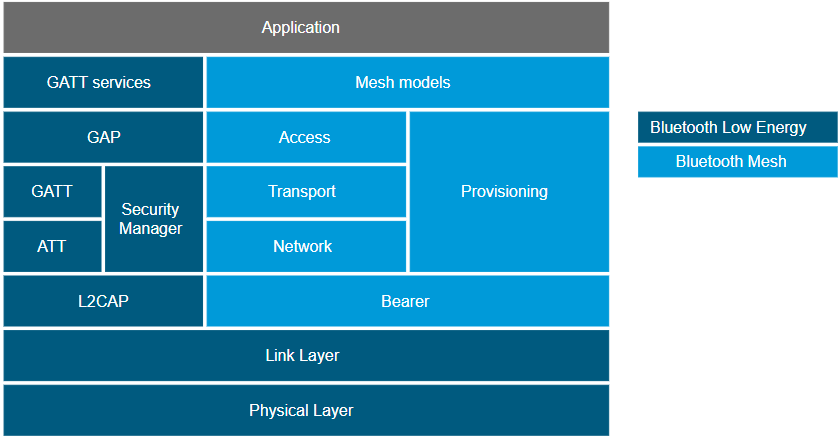
\includegraphics[width=11cm]{images/Bluetooth-mesh-vs-BLE.png}
        		\caption{Mối quan hệ giữa Bluetooth mesh và BLE}
        	\end{center}
        \end{figure}
        \subsection{Sứ mạng của Bluetooth Mesh}
        Bluetooth Mesh hướng đến những ứng dụng điều khiển hoặc giám sát cần các kết nối nhiều:nhiều (một mạng mesh có khả năng phân tán tốt), số thiết bị có thể lên đến hàng ngàn, theo Nordic thì Bluetooth Mesh hỗ trợ tối đa 32767 thiết bị trong một mạng (con số này dựa trên trường địa chỉ mà giao thức BLE Mesh hỗ trợ) với đường kính mạng tối đa là 127 hops\cite{meshconcept}. Chính Nordic đã thử nghiệm trên hệ thống hơn 1000 thiết bị và đạt kết quả khả quan.\\
        
        Định dạng gói tin được tối ưu hóa cho các gói tin nhỏ (kiểu short-burst) chẳng hạn như tắt mở thiết bị, giá trị của số vài cảm biến, giá trị độ sáng bóng đèn,... không dành cho việc truyền dữ liệu hoặc các ứng dụng băng thông cao khác như streaming nhạc và video.
        \begin{figure}[h!]
        	\begin{center}
        		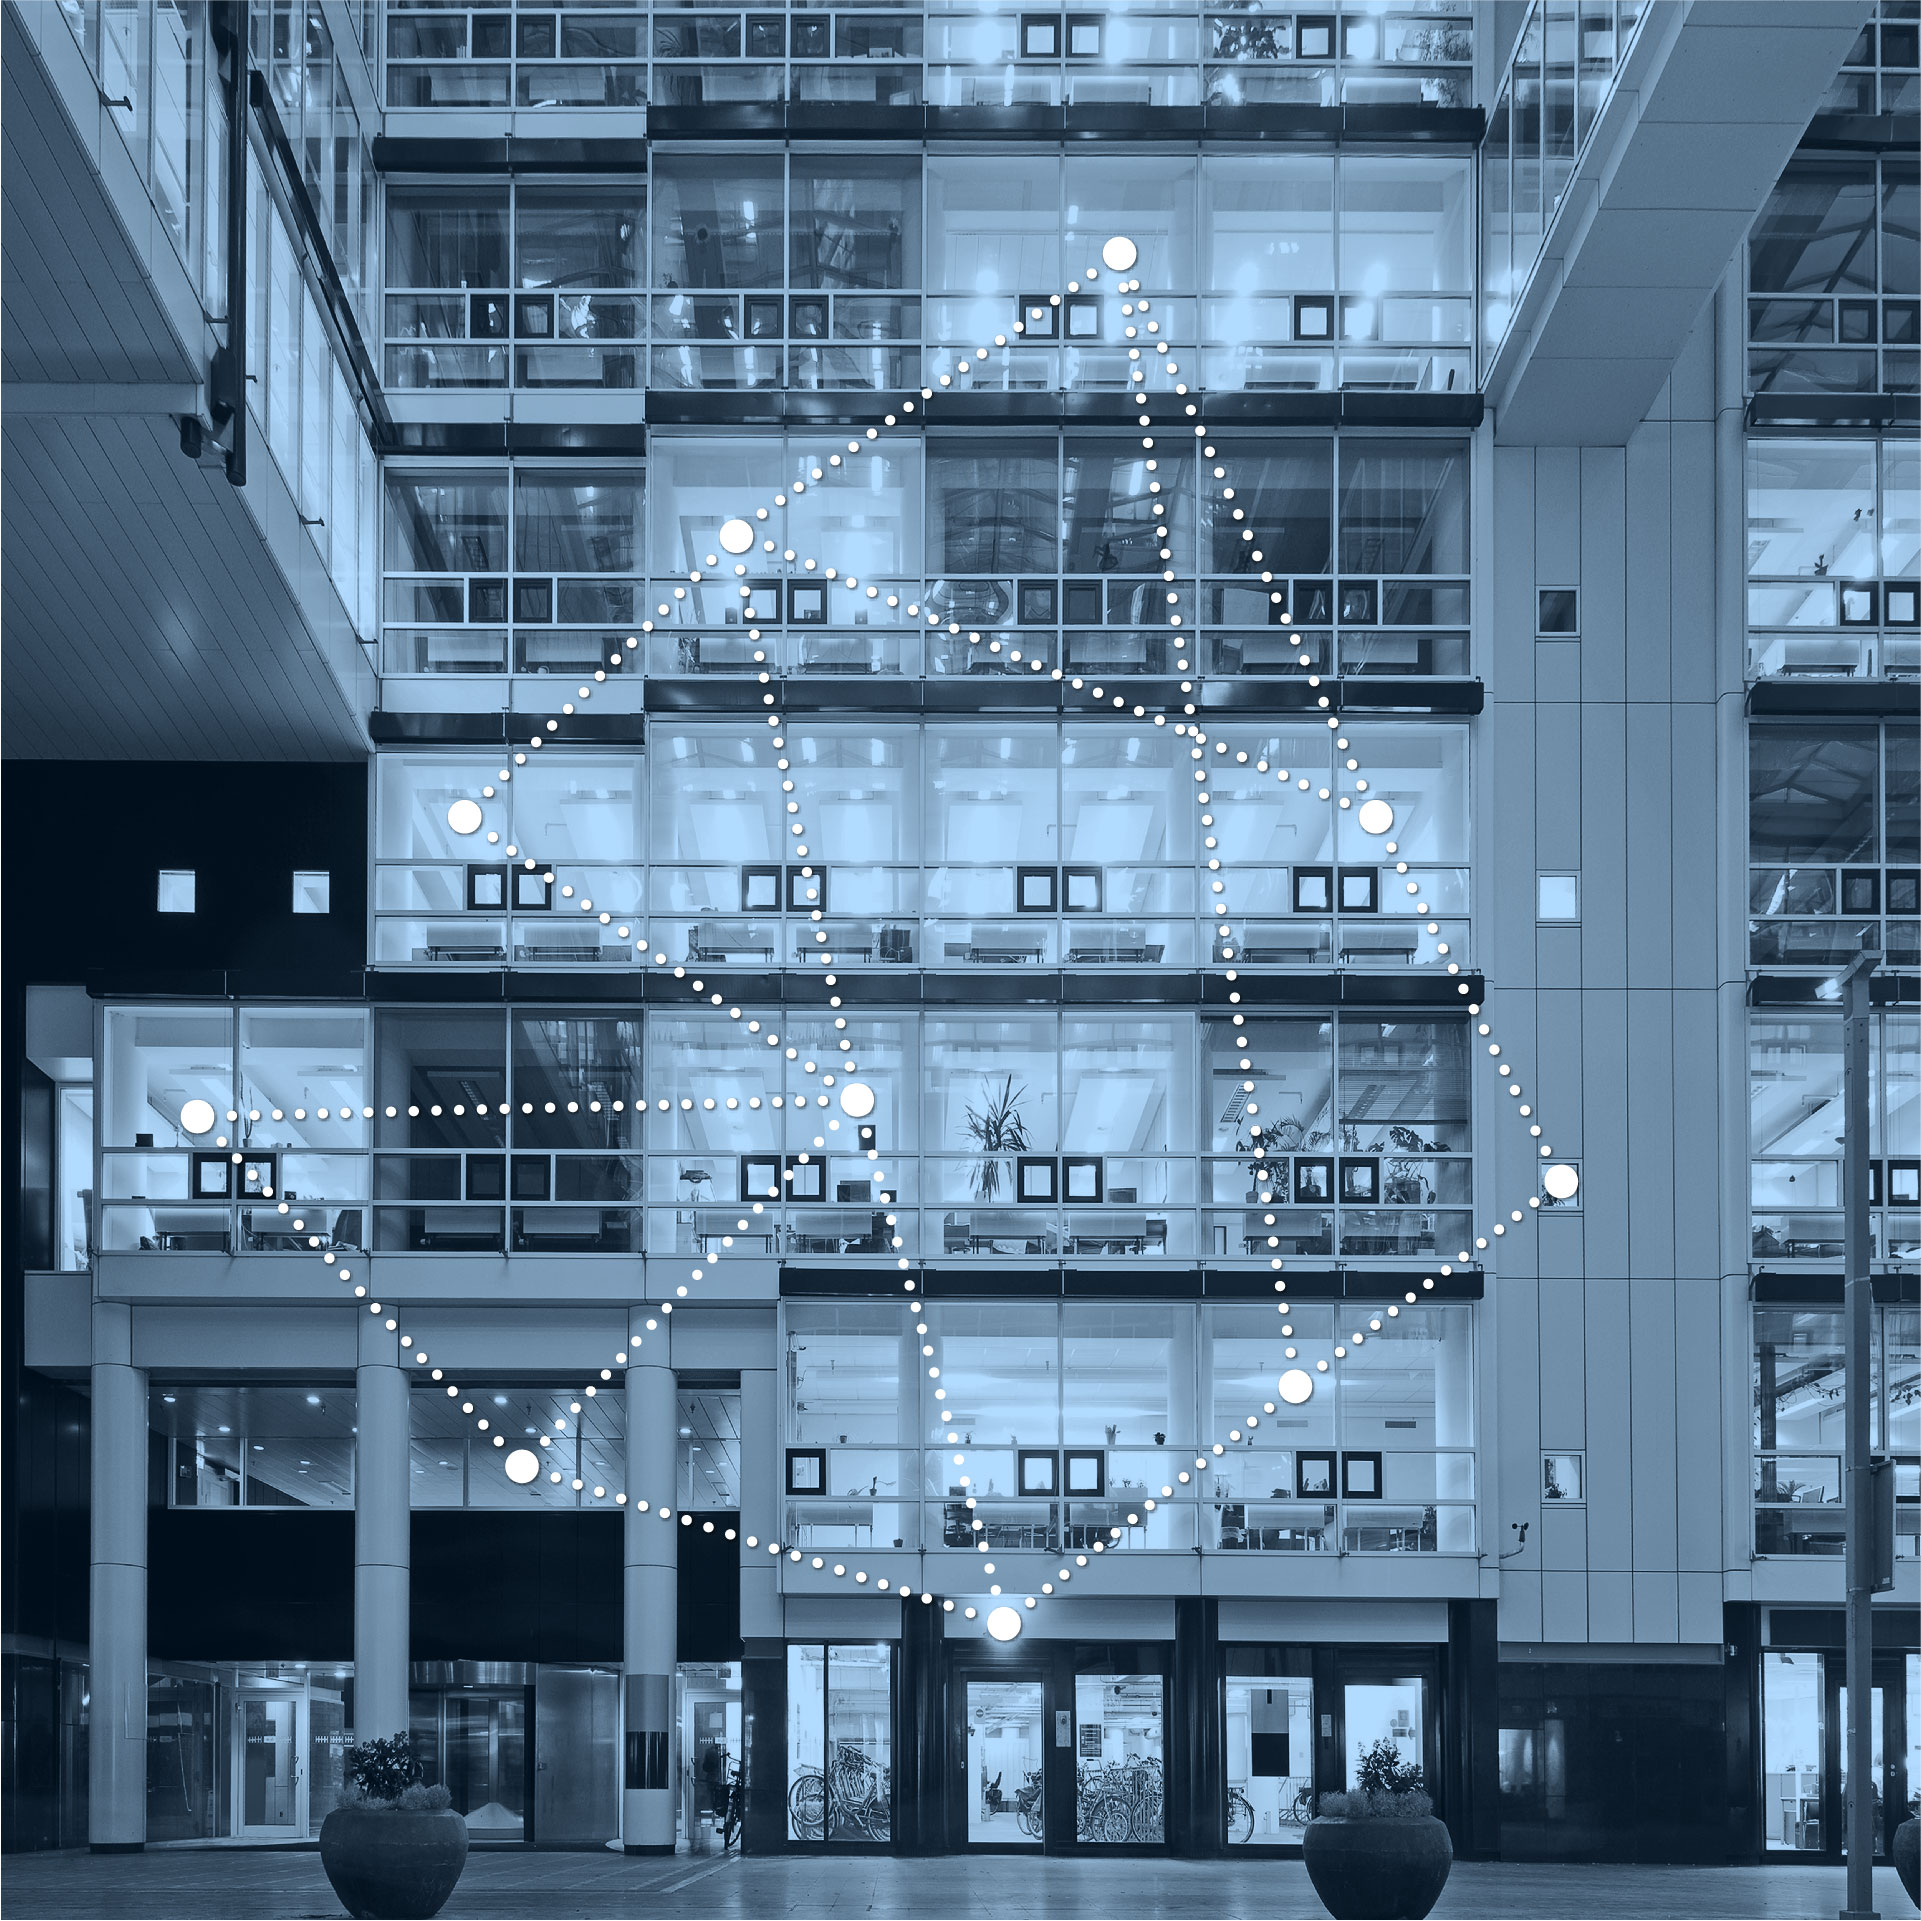
\includegraphics[scale=0.2]{images/Office_4_square_LE-mesh.jpg}
        		\caption{Hệ thống đèn của một tòa nhà ứng dụng Bluetooth Mesh}
        	\end{center}
        \end{figure}
        
    \section{Ưu điểm của Bluetooth Mesh}
    Để tiến hành triển khai các ứng dụng IoT trong thực tế, vấn đề bảo mật là cực kỳ quan trọng, đặc biệt trong các ngành y tế, giao thông và an ninh, hiện nay các hệ thống IoT sử dụng các giao thức thông thường như WiFi, Ethernet, GSM bị xem là bảo mật kém. Kể cả trong các ứng dụng điều khiển trong nhà thì việc một người lạ có quyền tắt mở đèn, quạt trong nhà của chúng ta thì cũng đủ mang lại nhiều phiền phức rồi. \\
    
    Vấn đề liên kết giữa các nhà sản xuất cũng quan trọng không kém, chẳng hạn chúng ta mua một bộ gồm đèn và remote của hãng A, sau một thời gian thì thấy đèn của hãng ko bền nên muốn dùng đèn của hãng khác, nhưng remote của hãng A lại không điều khiển được đèn của hãng khác mà mua một remote khác thì tốn kém hơn mua đèn nhiều.\\
    
    Ngoài ra còn hai vấn đề không kém phần quan trọng là tính mở rộng và khả năng tiết kiệm năng lượng, tuy nhiên hai vấn đề này lại phụ thuộc vào các ứng dụng thực tế, một số ứng dụng thì cần nhưng một số lại không. Chẳng hạn như những hệ thống nhỏ, có số lượng thiết bị không đáng kể thì không cần thiết có khả năng mở rộng; những ứng dụng như hệ thống đèn có khả năng kết nối trực tiếp với mạng điện lưới thì tiết kiệm năng lượng trở nên không mấy quan trọng.\\
    
     \textbf{Bluetooth Mesh là giải pháp hội đủ cả bốn tiêu chí trên, rất thích hợp để làm nền tảng triển khai các ứng dụng từ công nghiệp cho đến dân dụng.}
        \subsection{Tính bảo mật}
            \begin{itemize}
                \item Bluetooth Mesh dùng 3 key để mã hóa: Devive Key, Application Key và Network Key dùng để mã hóa gói tin ở lớp network và application. NetKey giúp chia một mạng mesh thành nhiều subnet, chẳng hạn như subnet trong nhà và subnet ngoài vườn, do tính năng relay gói tin được hiện thức ở lớp Network nên nếu không cùng NetKey thì không thể relay, nghĩa là khác subnet sẽ không truyền tin qua lại được. Như vậy một mạng mesh có thể dùng nhiều NetKey trong đó có một NetKey cho toàn mạng và nhiều NetKey cho các subnet. AppKey mã hóa ở 2 lớp trên cùng là Model và Foundation Model, do đó chỉ có người nhận mới đọc được gói tin ở lớp này.
                \item NetKey còn được dùng để tạo ra Privacy Key, key này dùng để xáo trộn header của gói tin khiến cho kẻ tấn công không thể xác định địa chỉ nguồn, địa chỉ nhận.
                \item Mỗi gói tin đều có trường authentication (một cách chứng minh gói tin này xuất phát từ một node trong mạng) dài 64-bits, có thể tăng thêm.
                \item Chống tấn công kiểu relay bằng cách bắt buộc chỉ số sequence phải thay đổi mỗi lần gửi tin, ngoài ra còn hỗ trợ thêm một trường nonce như một cách redundant, trường này sẽ được tạo mới mỗi khi gửi nhận tin dựa trên 2 thông số là Initialisation Vector (IV) index và chỉ số sequence. Mỗi khi bộ đếm sequence gần cạn kiệt (tràn số hoặc không thể tạo ra nonce mới, nonce mới ở đây yêu cầu phải khác tất cả nonce cũ), lúc này sẽ tiến hành quy trình cập nhật IV cũng tương tự quy trình tạo mới key chống trashcan dưới đây.
                \item Chống tấn công kiểu brute-force bằng độ dài key vào mạng 128-bits, trường authentication 64-bits.
                \item Chống tấn công kiểu man-in-the-middle (MITM) bằng cách áp dụng quy trình trao đổi key ECDH\cite{ECDH} cùng với out-of-band authentication (xác thực thông qua một bên thứ ba, có thể là một kênh giao tiếp khác).
                \item Chống tấn công kiểu trashcan: kẻ tấn công lấy thông tin như key vào mạng từ một node bị hỏng hoặc lỗi nên bị loại khỏi mạng. Cách thức chống kiểu tấn công này sẽ được thảo luận trong phần \ref{removenode}.
                \item Chống tấn công kiểu vật lý: vì Bluetooth Mesh hỗ trợ mạng lưới thiết bị rộng lớn nên không tránh khỏi việc một số node không an toàn về vật lý: đèn ở ngoài vườn có độ an toàn vật lý thấp hơn hẳn đèn trong phòng ngủ, do đó kẻ tấn công có thể khai thác lỗ hổng này bằng cách tấn công vào node kém an toàn và từ đó điều khiển toàn bộ mạng. Bluetooth Mesh có khả năng phân loại key: key dành cho nhóm kém an toàn khác với key của nhóm an toàn nên các node kém an toàn không điều khiển được các node an toàn.
                \item Chống tấn công kiểu visitor bằng cách cấp cho các node tạm (trong một số ứng dụng sẽ phát sinh các node cần truy cập tạm thời vào mạng để gửi nhận thông tin) key có thời gian sống giới hạn, sau một thời gian node tạm không còn khả năng truy cập mạng nữa.
                \item Ngoài ra các gói tin còn được xác thực bằng các thuật toán như AES-CMAC, AES-CCM,...
            \end{itemize}
        \subsection{Tính liên kết}
        Bluetooth Mesh có khả năng liên kết các nhà cung cấp với nhau. WiFi và Zigbee đang được sử dụng phổ biến trong các giải pháp mà Bluetooth Mesh dự định thay thế: smart building, smart home,... nhưng lại thiếu sự tương tác giữa các nhà cung cấp. Các thiết bị của hai hãng khác nhau không thể giao tiếp với nhau, do cấu trúc lệnh của mỗi hãng là do họ tự định nghĩa. Đối với Bluetooth Mesh thì khác, SIG đã định nghĩa sẵn các model như cách BLE đã làm với các profile chuẩn, các nhà sản xuất chỉ việc làm theo đúng chuẩn đó thì điều khiển hãng này dùng cho bóng đèn hãng khác không còn là vấn đề.
        \subsection{Dễ mở rộng}
        Do đặc thù là mạng mesh nên ưu điểm của Blueetooth Mesh sẽ là tính phân tán, các node không cần phải đặt tập trung vào một gateway hay access point mà có thể đặt bất cứ nơi đâu tùy theo nhu cầu ứng dụng. Khi áp dụng giao thức BLE Mesh vào trong IoT, phạm vi hoạt động của mạng lưới cảm biến sẽ được mở rộng rất nhiều, chẳng hạn như node A nằm ngoài phạm vi kết nối của node B, tuy nhiên chỉ cần đặt thêm node C vào giữa hai node này, thế là A có thể giao tiếp với B thông qua C, thử tưởng tượng với 127 hops mà khoảng cách giữa 2 node khoảng 8 - 10m (kết quả thử nghiệm thực tế), phạm vi tối đa sẽ đạt tới mức nào? 
        \subsection{Tiết kiệm năng lượng}
        Bluetooth Mesh là giao thức mạng, kết thừa các lớp của BLE nên cũng kế thừa khả năng tiết kiếm năng lượng. Ngoài ra, Bluetooth Mesh còn đưa ra khái niệm Friendship, giúp cho các node cần tiết kiệm năng lượng  có thể ở trạng thái sleep lâu hơn mà không bị loại ra khỏi mạng hoặc bỏ lỡ những gói tin được gửi tới nó. 
        \subsection{Một số ưu điểm khác của Bluetooth Mesh}
        \begin{itemize}
            \item Bluetooth Mesh đạt các yêu cầu cho một ứng dụng công nghiệp với đầy đủ các yêu cầu: đáng tin cậy (reliability), dễ mở rộng (scalability) và tính bảo mật cao.
            \item Sản phẩm dễ được thị trường đón nhận hơn vì Bluetooth đã trở thành thường thức với phần đông dân số thế giới, do đó khi nhà sản xuất miêu tả sản phẩm này áp dụng giao tiếp Bluetooth thì khách hàng dễ hình dung hơn là Zigbee hay Lora nhiều.
            \item Chức năng Bluetooth vốn tích hợp sẵn trên mọi chiếc điện thoại thông minh, thậm chí điện thoại không thông minh, cũng như rất nhiều thiết bị công nghệ như máy tính bảng, laptop,... Mức độ phổ biến của nó tương ứng với tiềm năng phát triển trong tương lai, khi mà Bluetooth Mesh chấp nhận giao tiếp với thiết bị non-mesh (các thiết bị dùng Bluetooth hiện nay đều là non-mesh), mà theo như thông tin nhóm tìm hiểu thì các một số thiết bị BLE từ 4.0 trở lên và có đủ điều kiện (chẳng hạn như dung lượng bộ nhớ còn trống trong chip) thì có thể giao tiếp với một mạng mesh thông qua ứng dụng.
            \item Khi mạng lưới càng lớn thì khả năng tự hồi phục của mạng càng mạnh, việc một vài node bị hỏng sẽ không ảnh hưởng tới mạng bất kể node đó có phải relay hay không, bởi vì còn rất nhiều con đường khác - những node relay khác - để gói tin có thể đi qua.
            \item Khả năng thiết lập kết nối nhanh, khi có phần tử mới muốn tham gia vào mạng, chỉ cần được thiết lập với key hợp lệ.
            \begin{figure}[h!]
        	    \begin{center}
        		    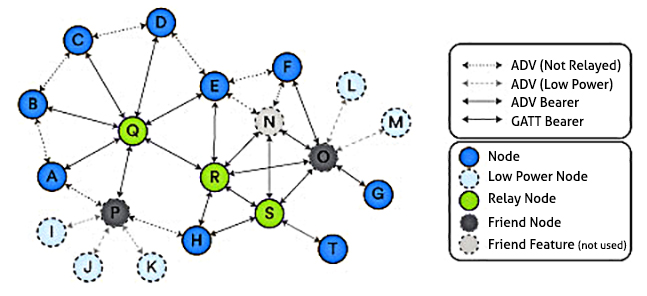
\includegraphics[scale=1.0]{images/mesh-topo.jpg}
        		    \caption{Mạng mesh với node "bạn bè" và low power}
        	    \end{center}
            \end{figure}
        \end{itemize}
        \newpage
    \section{Kiến trúc Bluetooth Mesh}
    Trong phần này, nhóm sẽ trình bày những đặc điểm chính của từng thành phần trong kiến trúc Bluetooth Mesh. Mô hình kiến trúc được thể hiện trong hình bên dưới:
    
    \begin{figure}[h!]
    	\begin{center}
    		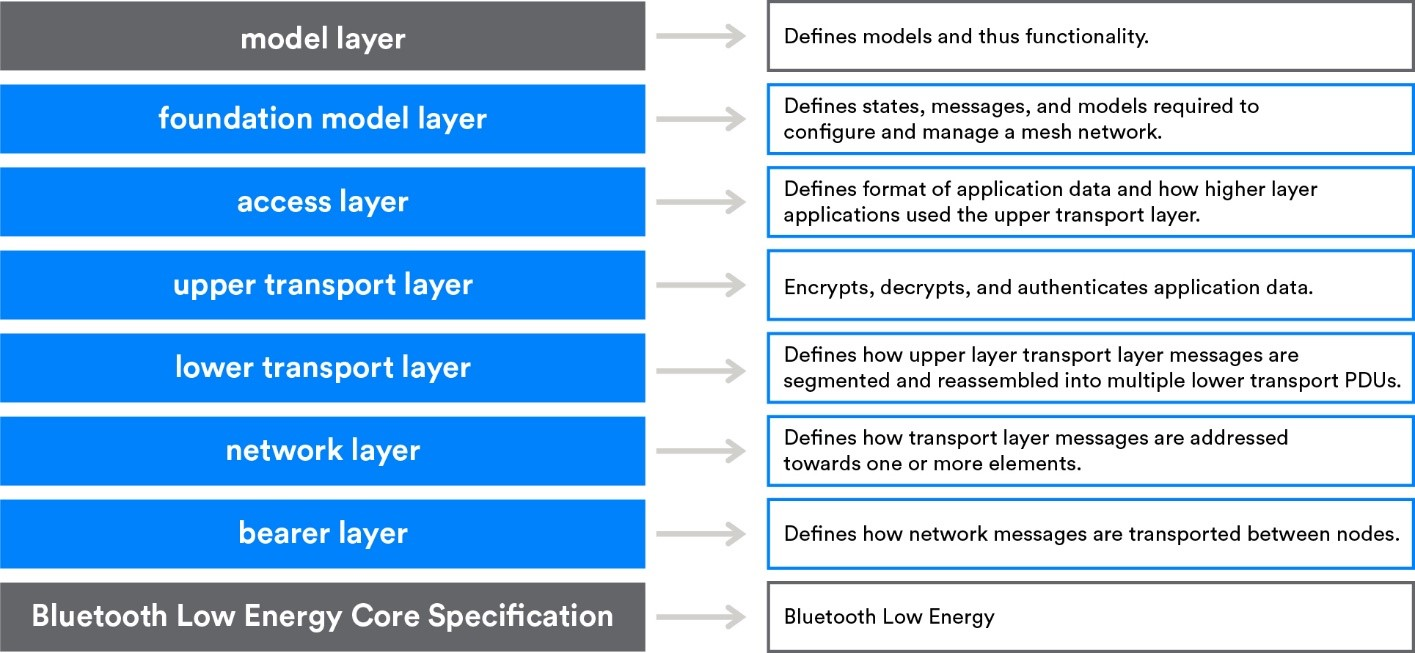
\includegraphics[scale=0.8]{images/mesh-architexture.jpg}
    		\caption{Kiến trúc Bluetooth mesh}
    	\end{center}
    \end{figure}
    
    \subsection{Lớp Model}
    Lớp model chịu trách nhiệm hiện thực các model, nghĩa là hiện thực các hành vi, trạng thái, gói tin điều khiển,... Tham khảo thêm về các model chuẩn trong phần phụ lục \ref{models}.
    \subsection{Lớp Foundation Model}
    Lớp Foundation Model như một lớp đệm cho lớp Model, thiết lập và quản lý lớp Model cho thích hợp với mạng mesh.
    \subsection{Lớp Access}
    Lớp Access kết nối và giúp 2 lớp trên (lớp Model và Foundation Model, nếu gộp 2 lớp này lại thì giống với lớp Apllication trong mô hình OSI) sử dụng tài nguyên là các lớp bên dưới.
    \begin{itemize}
        \item Định nghĩa cấu trúc của 2 lớp trên
        \item Định nghĩa và điều khiển quá trình mã hóa, giải mã trong lớp Upper transport
        \item Kiểm tra và xác nhận gói tin được gửi từ lớp Upper transport là đúng mạng và đúng ứng dụng trước khi chuyển lên lớp cao hơn
    \end{itemize}
    \subsection{Lớp Upper Transport}
    Lớp Upper transport chịu trách nhiệm mã hóa, giải mã và xác thực gói tin chuyển xuống (lúc gửi) hoặc trước khi chuyển lên (lúc nhận) lớp Access. Lớp này cũng chịu trách nhiệm tạo ra và vận chuyển các gói tin đặc biệt qua lại giữa các node: bao gồm các gói tin liên quan đến friendship và heartbeats.
    \subsection{Lớp Lower Transport}
    Lớp Lower transport nhận gói tin từ lớp Upper transport layer và chia nhỏ nếu gói tin quá dài, vượt quá giới hạn của lớp này. Trong trường hợp nhận, lớp Lower transport sẽ chịu trách nhiệm ghép gói tin lại nếu nó đã bị chia nhỏ, sau đó chuyển lên lớp trên.
    \subsection{Lớp Network}
    Lớp Network định nghĩa các kiểu địa chỉ (unicast, vitural, group) cũng như cấu trúc của gói tin ở lớp này, cho phép gói tin từ lớp Transport đi xuống lớp Bearer. Lớp này hỗ trợ nhiều bearer (một dạng kênh truyền), trong đó mỗi bearer lại mang nhiều network interface, network interface là cách để các element của các node giao tiếp với nhau, bao gồm cả các element trong cùng 1 node (local network interface). \\
    
    Lúc gửi dữ kiệu lớp Network layer sẽ quyết định gửi gói tin tới network interface nào, sau đó lớp này sẽ thông qua bộ lọc để lọc các dữ liệu được đưa xuống lớp Bearer. Lúc nhận gói tin từ lớp Bearer, một bộ lọc sẽ lọc xem gói tin nào sẽ được đưa tiếp lên lớp trên (khi đúng network interface), gói tin nào sẽ bỏ qua. Tính năng Relay và Proxy được hiện thực ở lớp Network.
    \subsection{Lớp Bearer}
    Các gói tin mesh cần một nền tảng để gửi nhận, nền tảng đó chính là BLE, lớp Bearer sẽ định nghĩa cách các gói tin được xử lý và vận chuyển. Hiện nay có hai Bearer là Advertising Bearer và GATT Bearer.\\
    
    Advertising Bearer kế thừa tính năng quảng bá (advertising) và dò tìm (scanning) của BLE GAP để gửi nhận các gói tin mesh. Còn GATT Bearer cho phép các thiết bị không hỗ trợ Advertising Bearer giao tiếp gián tiếp với các node trong mạng mesh thông qua giao thức Proxy. Node sử dụng giao thức này gọi là node Proxy, node sử dụng Proxy và node sử dụng Advertising Bearer có thể giao tiếp với nhau một cách bình thường.\\
    
    Giao thức Proxy sử dụng profile GATT vốn là profile cơ bản nhất của BLE, trong đó giao thức này sẽ sử dụng một số characteristics được định nghĩa sẵn để giao tiếp (Mesh Proxy Data). Gói tin sẽ được write vào characteristics Mesh Proxy Data In của node proxy, gói tin sẽ được lấy ra từ characteristics Mesh Proxy Out.
     \section{Nguyên lý hoạt động của Bluetooth Mesh}
            \subsection{Phần tử trong mạng}
            Mỗi thiết bị tham gia trong mạng được gọi là một node, trong một ứng dụng thực tế thì mỗi một node đều có thể có nhiệm giống hoặc khác nhau, chẳng hạn như node đọc giá trị cảm biến do tính chất đọc theo chu kỳ nên có thể dùng nguồn pin và chạy low power, node gateway lại cần cấp nguồn liên tục để cập nhật tình hình với server,... Trong mạng Bluetooth Mesh có 4 loại node đặc biệt như sau:
            \begin{itemize}
                \item Low-power: tiêu tốn năng lượng cực thấp, có thể hoạt động trong vòng vài năm với nguồn pin coin (coin battery).
                \item Friend: bắt buộc phải có nếu trong mạng có node low-power, bởi vì mỗi khi node low-power muốn giao tiếp, nó sẽ chỉ giao tiếp với node friend của nó, còn node friend có nghĩa vụ lưu lại những dữ liệu mà các node khác gửi cho node low-power. Do đó node friend cần cấp nguồn liên tục.
                \item Relay: node relay sẽ broadcast bất cứ dữ liệu nào được gửi đến nó mà nó ko phải người nhận duy nhất, giúp mở rộng mạng mesh. Node relay cũng cần cấp nguồn liên tục.
                \item Proxy: node này liên kết các node trong mạng mesh với các thiết bị sử dụng BLE và không nằm trong mạng mesh, node proxy cũng cần năng lượng và thêm khả năng tính toán của vi xử lý.
            \end{itemize}
            \newpage
            Dù các node có hay không 4 chức năng trên, cấu trúc một node cũng gồm nhiều thành phần nhỏ hơn được thể hiện trong các hình sau:
            \begin{figure}[h!]
            	\begin{center}
            		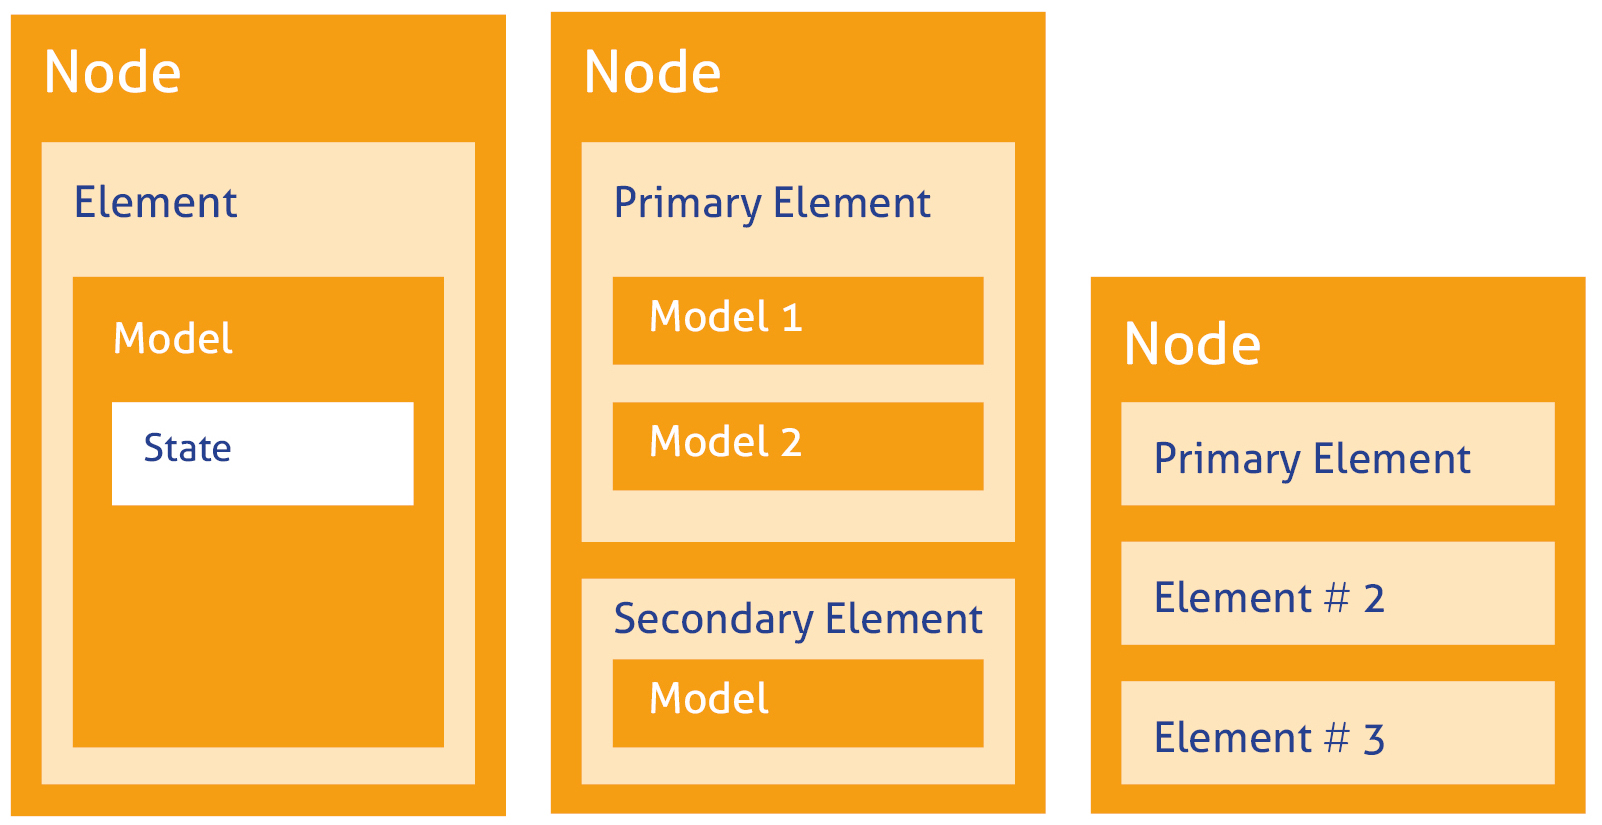
\includegraphics[scale=0.2]{images/mesh-node.jpg}
            		\caption{Cấu trúc của một node}
            	\end{center}
            \end{figure}

            Mỗi node phải gồm ít nhất một element - element sẽ định nghĩa các state (trạng thái) hoặc chức năng (functionality) của node. Ví dụ một node điều khiển nhiều thiết bị, các thiết bị là các element và mỗi element lại có nhiều trạng thái khác nhau, mỗi trạng thái là một model (model server). Hình bên dưới minh họa element đèn bao gồm 2 model trạng thái đèn và model độ sáng đèn.
            \begin{figure}[h!]
            	\begin{center}
            		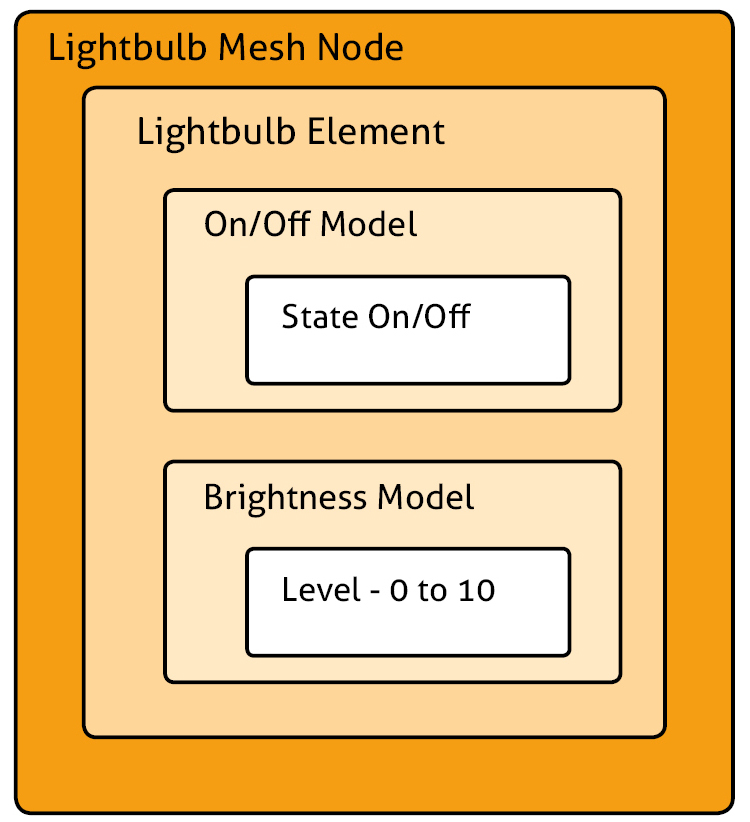
\includegraphics[scale=0.2]{images/lighbulb-node.jpg}
            		\caption{Cấu trúc của một node bóng đèn}
            	\end{center}
            \end{figure}

            Các model trong giao thức Bluetooth Mesh được phân làm 3 loại:
            \begin{itemize}
                \item Server: thể hiện trạng thái, như trong ví dụ trên. Sau đó nhận tin từ các node khác để thay đổi trạng thái và xuất tín hiệu ra các chân I/O, PWM tương ứng.
                \item Client: thể hiện chức năng, bao gồm các hàm có chức năng thay đổi trạng thái của các model server.
                \item Control: thể hiện cả trạng thái và chức năng, cộng thêm liên hệ logic giữa trạng thái và chức năng. Ví dụ một model control quạt dựa vào nhiệt độ, model này có chức năng lấy dữ liệu nhiệt độ từ cảm biến (của một node khác), sau đó kiểm tra ngưỡng rồi quyết định bật hay tắt quạt.
            \end{itemize}

            Trong đề tài này node gateway sẽ dùng model Simple OnOff client, node cảm biến sẽ dùng model Simple OnOff server. Node cảm biến lưu giữ trạng thái đèn (nhóm đã cải tiến thành lưu giữ giá trị cảm biến, xem phần \ref{simpleonoff}), node gateway sẽ đọc dữ liệu này để gửi lên server, nhóm có hiện thực thêm chức năng client gửi tín hiệu tắt/mở LED để tiện demo. Do đó có hiện tượng cùng một biến 8-bits nhưng có lúc lưu giữ giá trị cảm biến, có lúc lưu trạng thái đèn.
            \subsection{Truyền tin trong mạng}
            Bluetooth Mesh dùng cơ chế flooding để lan truyền gói tin, nghĩa là gói tin cần gửi sẽ được boardcast ra các node xung quanh, các node được boardcast sẽ kiểm tra mình có phải người nhận hay không, nếu không thì tiếp tục boardcast (còn gọi là relay, các node relay cần cung cấp nguồn đầy đủ và liên tục) cho đến khi tới được người nhận nếu là địa chỉ là unicast (hoặc một nhóm nhận nếu là địa chỉ multicast). Quá trình flooding này dừng lại khi đạt giới hạn 127 hops hoặc vượt quá thông số Time To Live (TTL) - thông số này tương đương số lần gói tin được relay\cite{meshgloss}.\\
            Sau đó, Bluetooth Mesh dùng cơ chế publish-subscribe để các gói tin tới được nơi cần tới. Các địa chỉ unicast được đánh cho các element trong node và được gọi là publish address, còn có multicast address và vitural address bao gồm nhiều element (địa chỉ multicast thường đại diện cho cho một tầng lầu, một phòng,... trong thực tế). Khi có tin mới được gửi đến một địa chỉ publish address, bất kỳ những model nào (element bao gồm nhiều model) trong element và có đăng ký nhận tin (subscribe) ở địa chỉ đó sẽ nhận được tin.
        
            \begin{figure}[h!]
        	    \begin{center}
        		    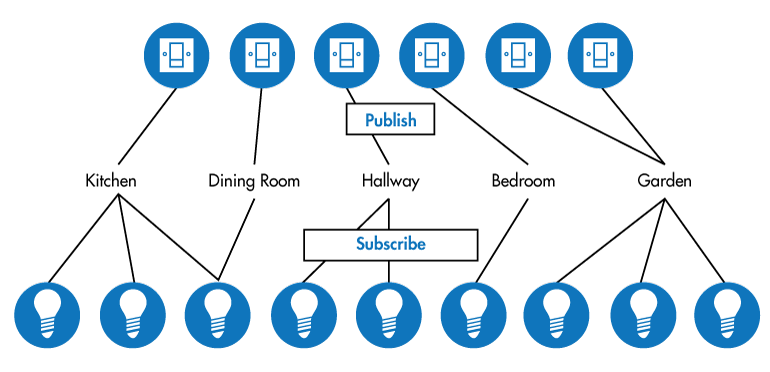
\includegraphics[scale=0.5]{images/mesh-pub-sub.png}
        		    \caption{Sơ đồ của cơ chế publish-subscribe}
        	    \end{center}
            \end{figure}
    \section{Quản lý các phần tử trong mạng}
        \subsection{Tham gia mạng - Provisioning}
            Để một thiết bị mới tham gia vào mạng mesh, cần thực hiện quá trình provisioning. Đây cũng được xem như quá trình bắt tay giữa các thiết bị khi tham gia vào mạng mesh, sau khi hoàn thành quá trình provionsing gồm 5 bước, thiết bị chính thức trở thành node - một thành phần trong mạng. Bluetooth Mesh hỗ trợ hai cách để provision một thiết bị:
            \begin{itemize}
                \item PB-ADV: Sử dụng gói advertising của BLE để tiến hành provisioning bằng cách thay đổi một số trườngww.
                \item PB-GATT: Sử dụng các characteristics của GATT để tiến hành provisioning, chỉ dùng khi thiết bị mới không hỗ trợ advertising hoặc không cho tùy chỉnh gói advertising.
            \end{itemize}

            Ngoài ra, khi thiết bị mới nằm ngoài tầm phủ sóng của provisioner, Bluetooth cũng hỗ trợ provisioning thông qua các node trung gian hoạt động như các relay để gửi các gói tin liên quan provisioning, quá trình này gọi là remote provisioning. Quá trình này có thể không cần thiết trong đa số ứng dụng trong thực tế vì người dùng hoàn toàn có thể mang theo thiết bị provionser như smartphone, sau đó đặt thiết bị mới vừa tầm và tiến hành provisioning. Có thể tham khảo flowchart của quá trình này trong phần \ref{remoteprov}.

            \begin{figure}[h!]
            	\begin{center}
            		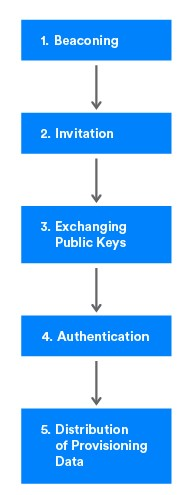
\includegraphics[scale=0.8]{images/mesh-management-fig2.jpg}
            		\caption{Quá trình provisioning gồm 5 bước}
            	\end{center}
            \end{figure}

            Tiếp theo, nhóm sẽ trình bày chi tiết hơn về quá trình provisioning thông qua PB-ADV:
            \begin{itemize}\label{security}
                \item Bước 1 - Beaconing: Khi một thiết bị mới (unprovisioned) muốn gia nhập mạng mesh, thiết bị này sẽ cần Network Key của mạng đó, sau đó tiến hành phát beacon để thông báo sự hiện diện của mình, tùy nhà sản xuất mà quá trình có thể kích hoạt bằng cách nhấn hoặc giữ nút,... Lúc này thiết bị đóng vai trò provisioner - thường sẽ là điện thoại, máy tính bảng có cài ứng dụng đặc biệt - sẽ tiến hành scan thiết bị mới, khi provionser phát hiện được thiết bị mới thì tiến hành bước tiếp theo. Trong đề tài này, nhóm sử dụng node gateway để thực hiện chức năng provisioning vì chưa phát triển được ứng dụng trên điện thoại.
                \item Bước 2 - Invitation: Provisioner sẽ gửi một lời mời, một gói tin Provisioning Invite PDU, đến thiết bị cần provisioning, thiết bị này sẽ đáp lại bằng một gói Provisioning Capabilities PDU, trong đó chứa một số thông tin của nó như số element,... đặc biệt là các input output mà nó hỗ trợ để tiến hành authentication sau này.
                \item Bước 3 - Exchanging Public Keys: Thiết bị mới và provisioner sẽ tiến hành trao đổi public key để dùng cho 2 bước cuối cùng của quá trình provisioning áp dụng giải thuật mã hóa bất đối xứng FIPS P-256 Elliptic Curve Algorithm. Quá trình trao đổi này có thể dùng phương pháp out-of-band để tăng tính bảo mật, out-of-band bao gồm các cách như quét QR code,...
                \item Bước 4 - Authentication: Sau khi biết được các input output mà thiết bị mới hỗ trợ nhờ bước 2, provisioner sẽ gửi yêu cầu sử dụng một trong các phương thức output, chẳng hạn như màn hình LCD hoặc LED, để thể hiện một hoặc nhiều con số (giống với mã PIN khi kết nối Bluetooth giữa 2 điện thoại). Người dùng sẽ quan sát và nhập con số này vào ứng dụng, provionser sẽ gửi và thiết bị mới sẽ kiểm tra để hoàn thành bước này (input/output authentication), hoặc đơn giản hơn là định nghĩa sẵn một dạng mật khẩu nào đó và để 2 bên xác thực bằng mật khẩu này (static authentication). Quá trình kiểm tra này có áp dụng hash để bảo mật.
                \item Bước 5 - Distribution of the Provisioning Data: Provionser sẽ gửi Network Key và cấp Unicast Address cho các element (quá trình này sẽ áp dụng giải thuật mã hóa FIPS P-256 Elliptic Curve), lúc này thiết bị mới đã chính thức trở thành node - một thành viên trong mạng mesh.
                \item Nếu có lỗi xảy ra trong quá trình provisioning, kết nối giữa hai thiết bị sẽ bị hủy.
            \end{itemize}
	\newpage
            Sơ đồ dưới đây minh họa chi tiết hơn các bước của quá trình provisioning, dùng để tham khảo khi lập trình với Nordic Mesh SDK:
            \begin{figure}[h!]
            	\begin{center}
            		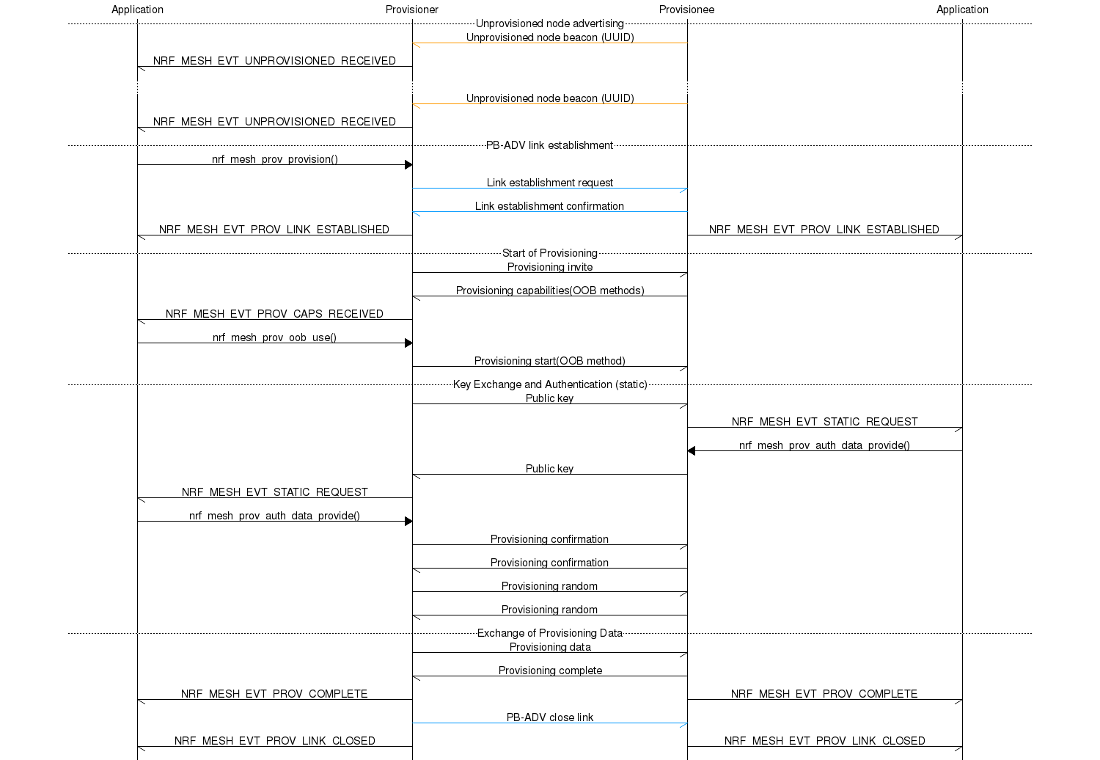
\includegraphics[scale=0.5]{images/provisioning.png}
            		\caption{Provisioning scenarios}
            	\end{center}
            \end{figure}

        \subsection{Thiết bị mới - Provisionee}
        Cách thức hoạt động của một thiết bị mới - unprovisioned hay provisionee: Tiến hành khởi tạo - bao gồm phát beacon để báo rằng mình cần tham gia provisioning, sau đó ở trạng thái chờ sự kiện. Khi bắt được sự kiện yêu cầu kết nối - lời mời provisioning từ provisioner thì đáp lại, tiếp đến chờ đáp lại các sự kiện xác thực, cuối cùng là kết thúc quá trình.
        \begin{figure}[h!]
        	\begin{center}
        		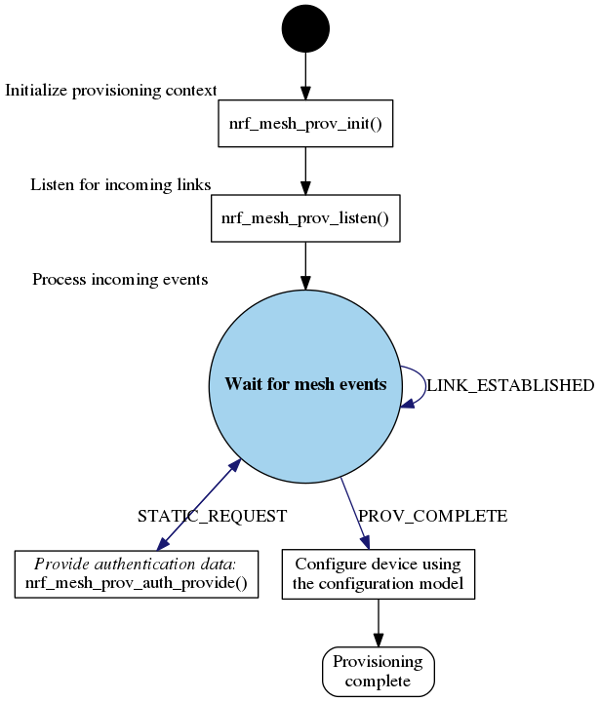
\includegraphics[scale=0.6]{images/provisionee_app_flowchart.png}
        		\caption{Provisionee flowchart}
        	\end{center}
        \end{figure}
	\newpage
        \subsection{Thiết bị Provisioner}
        Là thiết bị hoặc node chịu trách nhiệm thực hiện quá trình provisioning trong mạng mesh. Chúng thường là một phần của các thiết bị gateway - các thiết bị cung cấp một cầu nối giữa mạng mesh và các giao thức kết nối khác.  Cách thức hoạt động của một provisioner: sau các bước khởi tạo thì chờ beacon từ thiết bị mới (unprovisioned), sau đó mời tham gia quá trình provisioning. Trong bước xác thực, tùy theo đối tượng cần provisioning có hay không có hỗ trợ xác thực out-of-band (OOB) mà tiến hành xác thực theo cách tương ứng.
        \begin{figure}[h!]
        	\begin{center}
        		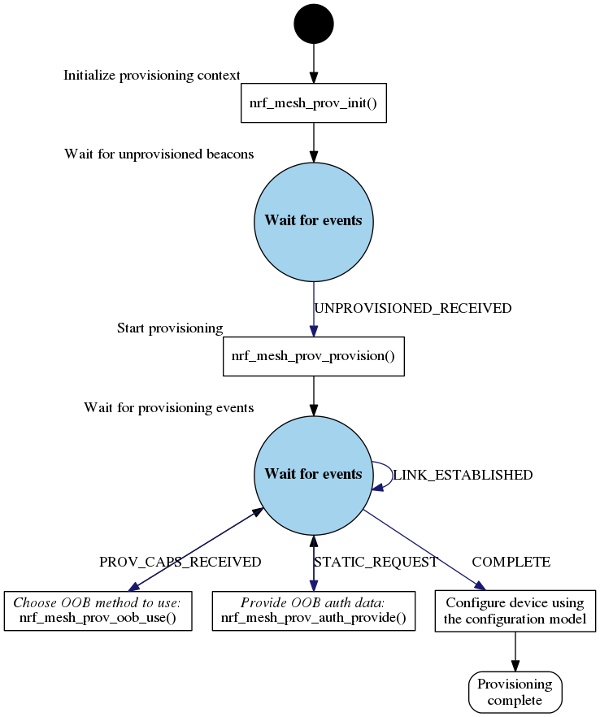
\includegraphics[scale=0.6]{images/provisioner_app_flowchart.png}
        		\caption{Provisioner flowchart}
        	\end{center}
        \end{figure}
        \subsection{Rời khỏi mạng} \label{removenode}
        Sau một thời gian hoạt động, việc phải loại bỏ một số node ra khỏi mạng là điều không thể tránh khỏi, có thể vì nhiều lý do như: node bị hỏng, chuyển node sang một khu vực khác với một mạng mesh khác, thay node mới,... Trong trường hợp nếu không có quy trình loại bỏ node, mạng sẽ đối mặt với nguy cơ bị tấn công kiểu Trashcan, kẻ tấn công có thể khai thác những node bị bỏ đi, lúc này chắc chắn lớp bảo vệ sẽ kém, để lấy thông tin và xâm nhập mạng. Bluetooth Mesh áp dụng 2 bước xử lý sau:
        \begin{itemize}
            \item Cho node bị loại bỏ vào danh sách đen.
            \item Tiến hành cấp lại NetKey cho các node trong mạng trừ node trong danh sách đen. 
        \end{itemize} 

        Quá trình này cần có một thời gian chuyển tiếp, trong thời gian này cả 2 key cũ và mới đều hợp lệ. Sở dĩ cần có thời gian chuyển tiếp này là vì các node low-power thỉnh thoảng mới hoạt động, do đó cần có thời gian để chúng nhận được chìa mới từ node friend của mình.
        \section{Khái niệm Friendship}
       Để có thể ở trong trạng thái sleep lâu dài, các node low power (LPNs) cần tiến hành thiết lập mối quan hệ Friendship với một node ``hàng xóm'' của mình, sau khi thiết lập xong thì node đó trở thành ``friend'' của LPN. Trước khi đi sâu hơn về khái niệm này, chúng ta cần làm quen với một vài tham số:
       \begin{itemize}
	\item ReceiveDelay: Khoảng thời gian từ lúc LPN gửi yêu cầu đến node friend cho đến lúc nó thức dậy lần nữa để bắt đầu nhận dữ liệu. Trong thời gian này LPN vẫn tiếp tục sleep, node friend thì tiến hành chuẩn bị dữ liệu để đáp lại yêu cầu đó.
	\item ReceiveWindow: Khoảng thời gian LPN thức dậy và lắng nghe, lúc này node friend mới có thể gửi dữ liệu cho LPN.
	\newpage
	\begin{figure}[h!]
        	\begin{center}
        		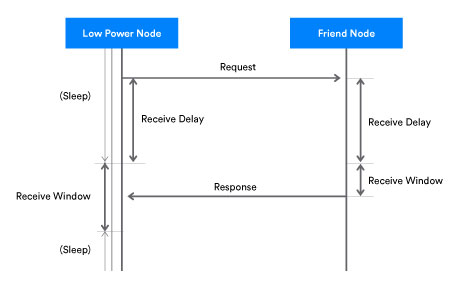
\includegraphics[scale=0.6]{images/friendship-1.jpg}
        		\caption{Hình mô tả ReceiveDelay và ReceiveWindow}
        	\end{center}
        	\end{figure}
        	\item PollTimeout: Khoảng thời gian tối đa giữa 2 lần LPN gửi yêu cầu cho node friend, nếu quá thời gian này mà vẫn không nhận được yêu cầu từ LPN, node friend sẽ kết thúc ``tình bạn'' với nó.
        	\begin{figure}[h!]
        	\begin{center}
        		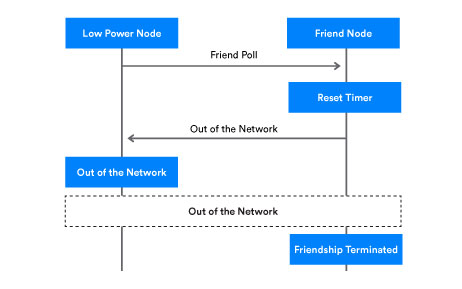
\includegraphics[scale=0.6]{images/friendship-2.jpg}
        		\caption{Hình mô tả PollTimeout}
        	\end{center}
          \end{figure}
       \end{itemize}
       \subsection{Các bước thiết lập Friendship}
       \begin{enumerate}
       \item Node LPN gửi ``yêu cầu kết bạn'', yêu cầu này sẽ không được relay vì nó chỉ có thể kết bạn với những node trong phạm vi kết nối của mình, ngoài ra các node trong phạm vi nhưng không hỗ trợ chức năng Friendship cũng sẽ bỏ qua yêu cầu này. Yêu cầu kết bạn này bao gồm cả 3 thông số ReceiveDelay, ReceiveWindow và PollTimeout.
       \item Node thỏa mãn các yêu cầu để trở thành Friend sẽ gửi lại Friend Offer cho LPN. Gói này bao gồm nhiều tham số như ReceiveWindow có thể hỗ trợ, sức chứa của buffer - buffer này để chứa ``hộ'' các dữ liệu được gửi tới LPN trong lúc nó ngủ và được gọi là Friend Queue,...      
       \item Khi LPN nhận được Friend Offer, nó sẽ dùng một thuật toán để chọn ra 1 Friend (nếu có nhiều Friend Offer), thuật toán này do người phát triển ứng dụng định nghĩa: có thể là ưu tiên node gần hơn hoặc node có khả năng hỗ trợ Friend Queue lớn hơn.
       \item Sau khi đã chọn được Friend, LPN gửi Friend Poll cho node đó.
       \item Sau khi nhận được Friend Poll, node Friend trả lời bằng Friend Update. Mối quan hệ Friendship chính thức được thiết lập.
       \end{enumerate}
       \subsection{Giao tiếp trong Friendship}
       Sau khi đã ``kết bạn'', LPN và node Friend của nó sẽ tiến hành giao tiếp theo các bước sau:
       \begin{figure}[h!]
        	\begin{center}
        		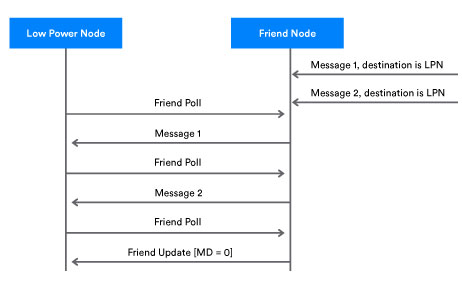
\includegraphics[scale=0.6]{images/friendship-3.jpg}
        		\caption{Hình mô tả quá trình giao tiếp}
        	\end{center}
          \end{figure}
       \begin{enumerate}
	\item Khi node Friend nhận được dữ liệu được gửi đến node LPN là ``bạn'' của nó, nó sẽ lưu vào Friend Queue. Trong hình trên, có thể thấy node Friend đã lưu lại Message 1 và Message 2 thay cho node LPN.
	\item Sau một chu kỳ ngủ, node LPN sẽ gửi yêu cầu Friend Poll đến cho node Friend của mình để kiểm tra có dữ liệu mới hay không.
	\item Nếu có dữ liệu mới, node Friend sẽ gửi ngược lại cho LPN, cứ mỗi lần LPN nhận được dữ liệu nó lại gửi thêm Friend Poll.
	\item Đến khi nào nhận được Friend Update (với tham số More Data = 0) nghĩa là không còn dữ liệu nữa, quá trình giao tiếp này sẽ kết thúc, LPN không gửi Friend Poll nữa.
      \end{enumerate}
      
      Các gói tin giữa node Friend và LPN đều được mã hóa bằng một loại key Friend và chỉ có 2 node này mới có khả năng đọc được.
\chapter{Thiết kế}

\section{Mô hình thiết kế}
    Với mục tiêu đề tài giúp các quadcopter bay được ổn định đồng thời vẫn giữ được trạng thái bầy đàn nhóm đề xuất ra mô hình bay như sau:
    \begin{itemize}
    	\item Mô hình sẽ có ít nhất hai chiếc quadcopter có thể hoạt động độc lập ổn định. Như vậy cần có các cảm biến cần thiết để triển khai phương pháp điều khiển PID cho quadcopter. Ngoài ra còn cần mạch thu phát sóng Wifi và một vi xử lý phụ nhằm xử lý dữ liệu bay.
    	\item Trạm điêu khiển mặt đất chạy phần mềm để thiết lập thông số các quadcopter đồng thời hiển thị dữ liệu và điều khiển các quadcopter bay theo các chế độ mong muốn.
    	\item Mỗi chiếc quadcopter kết nối với trạm điều khiển đồng thời trao đổi dữ liệu cảm biến qua lại với nhau nhằm tính toán để giữ đội hình bầy đàn.
    \end{itemize}
    
    \begin{figure}[h!]
    	\begin{center}
    		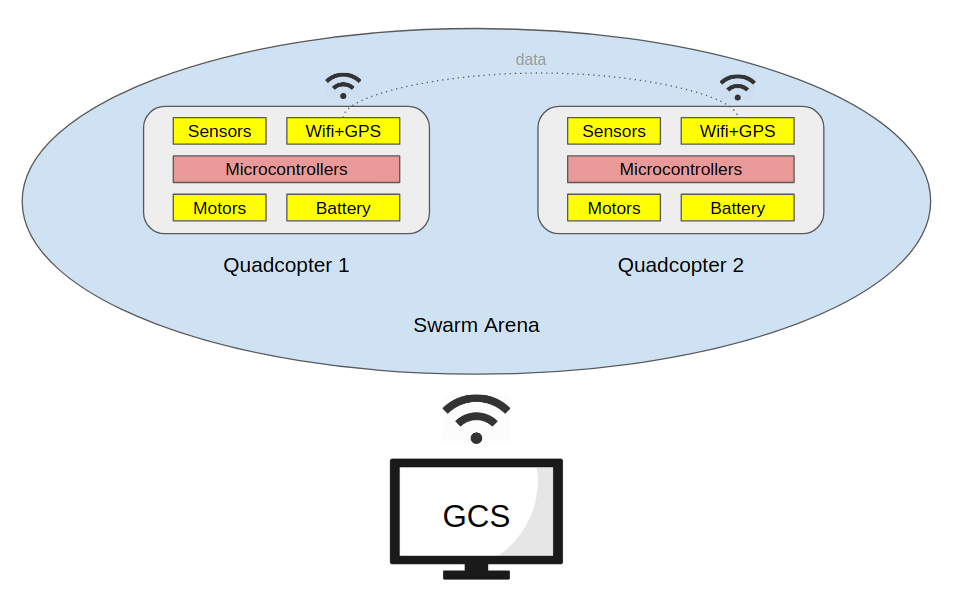
\includegraphics[scale=0.45]{images/design_model.png}
    		\caption{Mô hình thiết kế}
    	\end{center}
    \end{figure}
    
\section{Phần cứng} 
    \subsection{IMU - Đơn vị đo lường quán tính}
    Đơn vị đo lường quán tính là một thiết bị điện tử đo lường lực, tỷ lệ góc và đôi khi là từ trường bao quanh vật thể được dùng. IMU sử dụng kết hợp gia tốc kế, con quay hồi chuyển và từ kế. Nó là một thiết bị không thể thiếu cho các mô hình trên không bao gồm các thiết bị bay không người lái đặc biệt là quadcopter.\\
    Một bộ IMU khác biệt so với dùng các cảm biến riêng lẻ ở chỗ nó bao gồm những tập lệnh được thiết kế cho các phép tính toán ba chiều, tính toán hướng và góc. Mục đích chính là giảm tải thời gian và công suất xử lý cho bộ xử lý trung tâm. Kết quả trả về của nó có thể là giá trị analog hoặc digital đã tính toán tùy chỉnh.
    
    \begin{figure}[h!]
    	\begin{center}
    		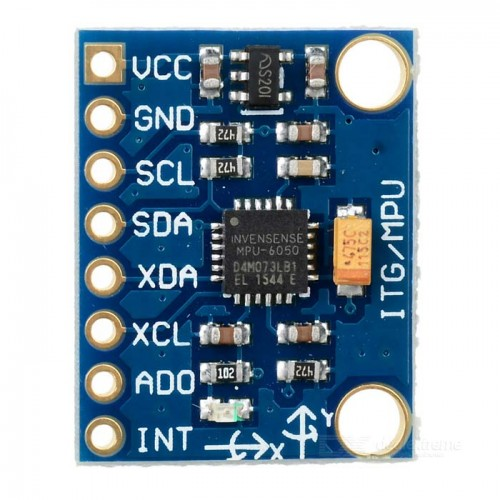
\includegraphics[scale=0.25]{images/mpu6050.jpg}
    		\caption{IMU MPU6050}
    	\end{center}
    \end{figure}
    
    \subsection{MCU - Vi điều khiển}
    Vi điều khiển luôn là bộ não trung tâm của bất kì thiết bị yêu cầu tính toán điện tử nào. Mục đích của vi điều khiển nhằm tạo một môi trường giao tiếp giữa các thiết bị ngoại vi, tính toán và đưa ra số liệu phù hợp để điều khiển các bộ phận giúp quadcopter bay được ổn định. Một vi điều khiển nhằm mục đích điều khiển bay cho quadcopter cần có khả năng xử lý năng lượng thấp, tốc độ xử lý nhanh và nhỏ nhẹ. Ngoài ra nếu muốn hỗ trợ tính toán từ các vi điều khiển khác thì vi xử lý cần có thêm nhiều cổng UART. \\
    Một bộ điều khiển bay Flight Controller là một bo mạch được thiết kế nhỏ gọn tích hợp vi điều khiển và các thiết bị ngoại vi cần thiết như IMU, GPS, ESC hay cảm biến khoảng cách và các cổng kết nối I2C, SPI hay UART. Flight Controller được xây dựng nhằm mục đích giúp người dùng dễ dàng tiếp cận với bộ firmware được xây dựng sẵn cho điều khiển bay cơ bản. Ngoài ra Flight Controller còn hỗ trợ tùy chỉnh thêm linh kiện và firmware cho phù hợp với mục đích sử dụng. \\
    Để đảm bảo quadcopter tính toán nhanh để ổn định mô hình bầy đàn, nhóm sử dụng thêm một vi xử lý phụ để xử lý giữ liệu bay cho các quadcopter.
    
    \begin{figure}[h!]
    	\begin{center}
    		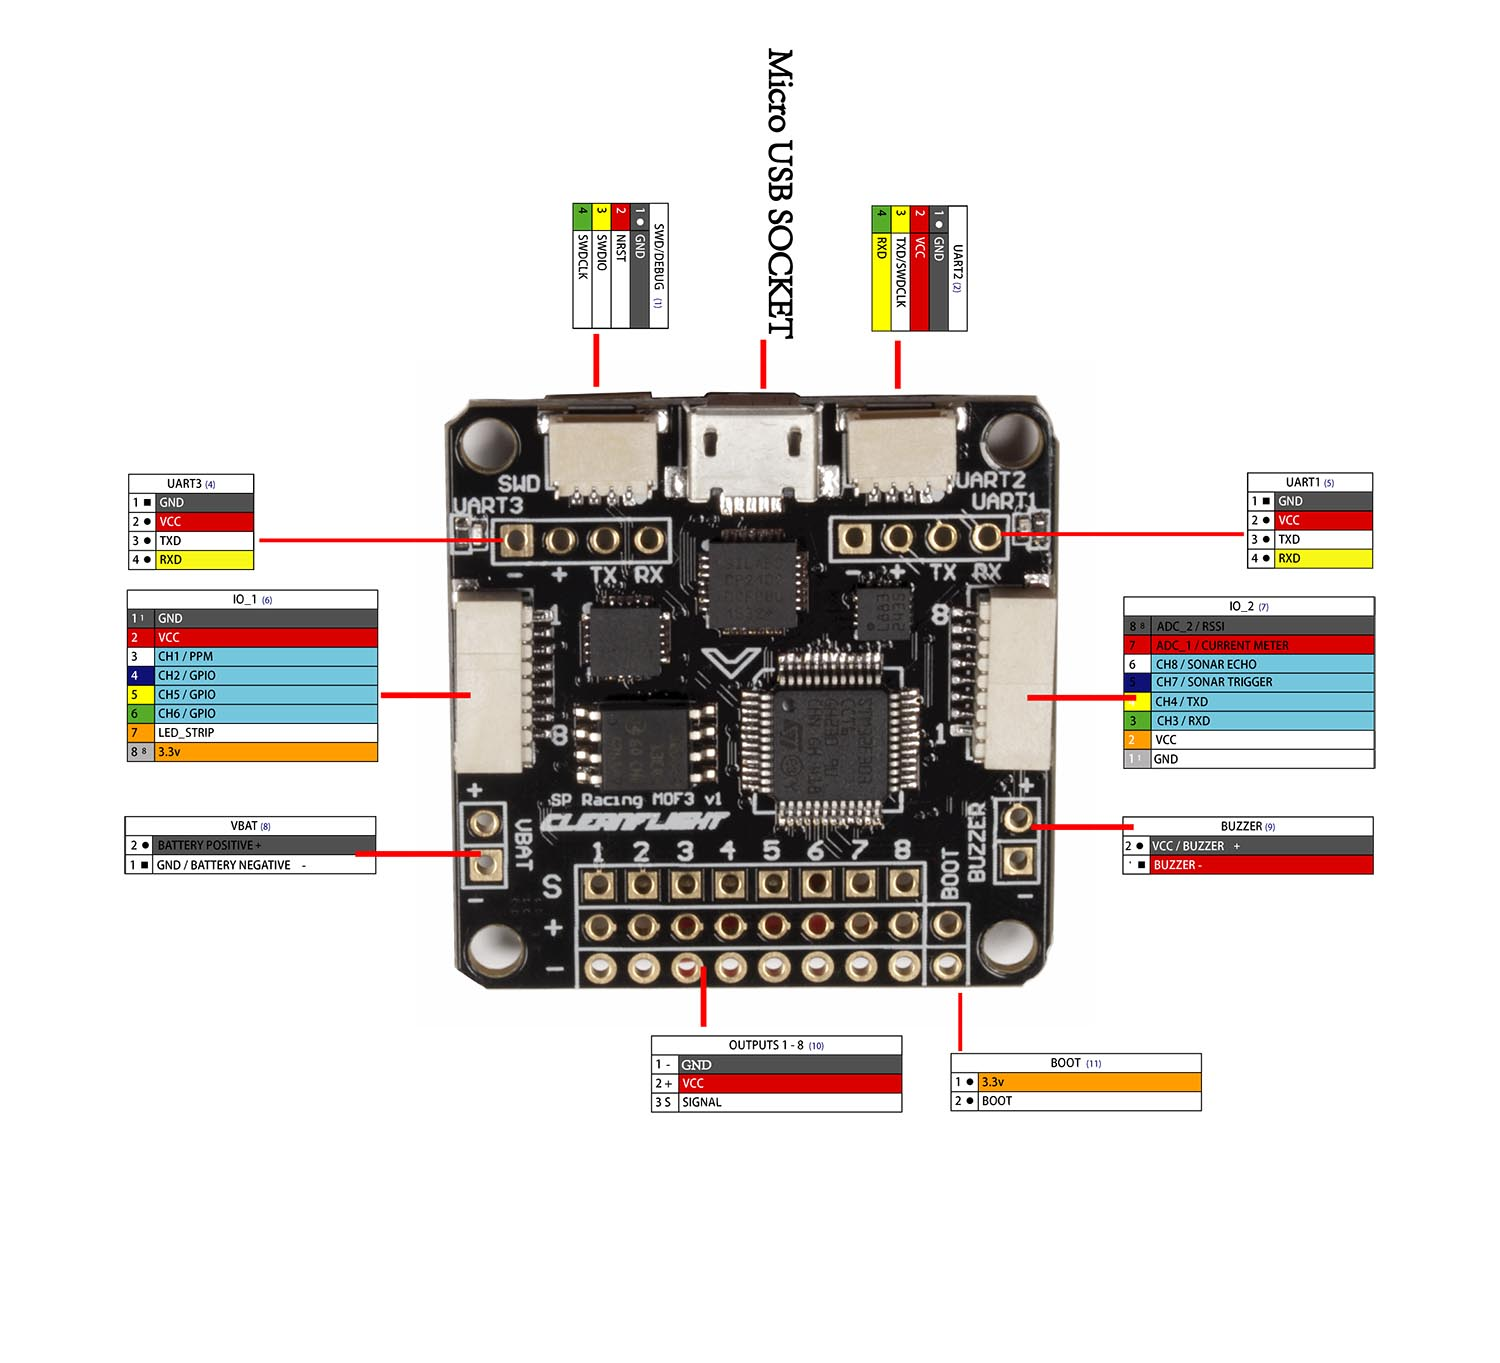
\includegraphics[scale=1.1]{images/sp_racing_f3.jpg}
    		\caption{Flight Controller SP Racing F3 Acro dùng vi xử lý STM32F303}
    	\end{center}
    \end{figure}
    
    \subsection{ESC - Bộ điều tốc}
    Bộ điều tốc ESC (Electronic Speed Control) là một bo mạch dùng nguồn điện ba pha điện áp thấp từ nguồn DC để thay đổi tốc độ động cơ không chổi than (brushless), chiều quay và cũng có thể sử dụng như thắng điện tử cho động cơ. Động cơ không chổi than là động cơ với công suất tiêu thụ cao chuyên dùng cho quadcopter hay những thiết bị cần công suất tiêu thụ cao khác và chạy với thời gian thực. 
    
    \begin{figure}[h!]
    	\begin{center}
    		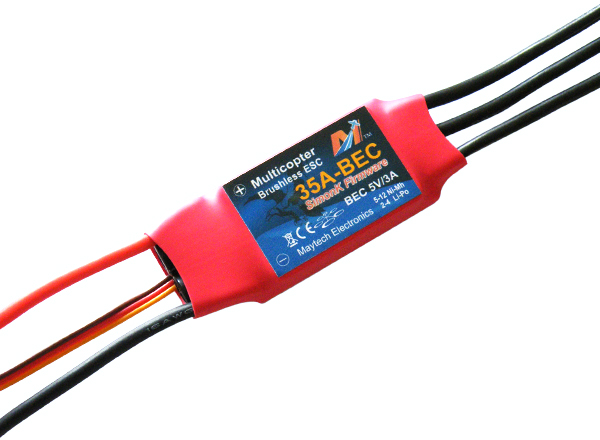
\includegraphics[scale=0.4]{images/esc.jpg}
    		\caption{Multicopter Brushless ESC 35A-BEC 5V/3A}
    	\end{center}
    \end{figure}
    
    \subsection{ESP8266}
    ESP8266 là dòng chip tích hợp Wi-Fi 2.4Ghz và một vi xử lý tốc độ 80MHz với chi phí thấp. ESP8266 vừa dùng để làm module giao tiếp giữa các quadcopter với nhau vừa có thể dùng để giao tiếp với trạm điều khiển mặt đất.

    \begin{figure}[h!]
    	\begin{center}
    		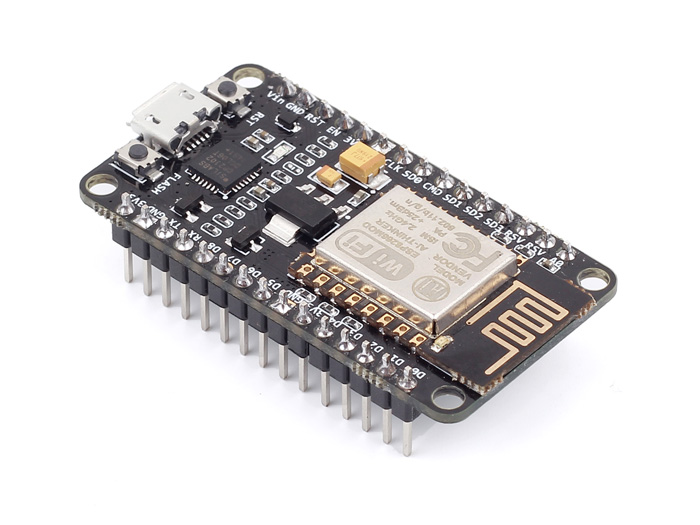
\includegraphics[scale=0.2]{images/esp8266.jpg}
    		\caption{NodeMCU ESP8266 WiFi ESP-12E}
    	\end{center}
    \end{figure}
    
    \subsection{Ultrasonic Sensor - Cảm biến siêu âm}
   Cảm biến sóng siêu âm được sử dụng rất phổ biến để xác định khoảng cách bởi giá thành rất rẻ và độ chính xác cao. Cảm biến siêu âm có thể đo khoảng cách trong khoảng từ 2cm đến 300cm dùng sóng siêu âm.
   Trong mô hình quadcopter, cảm biến siêu âm được xếp đều xung quanh quadcopter để giữ khoảng cách với vật cản và các quadcopter khác.
   
   \begin{figure}[h!]
    	\begin{center}
    		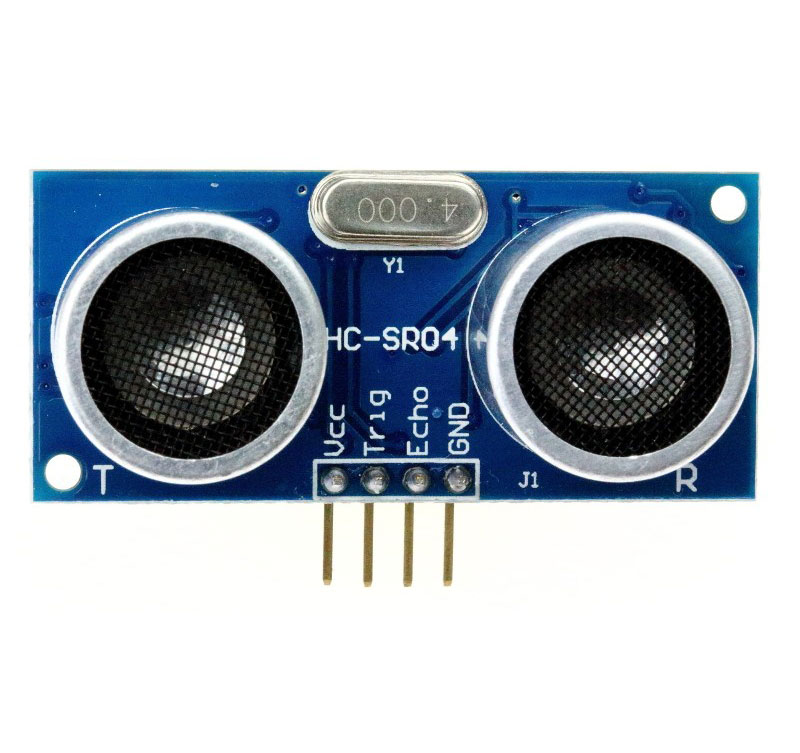
\includegraphics[scale=0.1]{images/ultrasonicsensor.jpg}
    		\caption{Ultrasonic Sensor HC-SR04}
    	\end{center}
    \end{figure}
   
    \section{Chương trình điều khiển và mô phỏng}
            \subsection{ArduCopter}
            ArduCopter là một hệ thống tự lái nâng cao mã nguồn mở cho các thiết bị bay dùng một hay nhiều rotor. Nó cung cấp nhiều chế độ bay từ thủ công cho đến bay hoàn toàn tự động.\\
            ArduCopter là một nhánh của chương trình rộng hơn ArduPilot cung cấp cho nhiều loại phương tiện bay trên không. Nó hoạt động liền mạch với chương trình điều khiển từ mặt đất được dùng để cài đặt phương tiện, hiển thị dữ liệu thời gian thực từ chuyến bay và lên kế hoạch bay cho phương tiện. Hệ sinh thái ArduPilot còn đem đến nhiều tính năng khác như mô phỏng bay, các công cụ phân tích nhật ký hành trình và các API nâng cao cho việc điều khiển phương tiện.\\
            Mục tiêu của nhóm là phát triển thêm chế độ bay theo bầy đàn dựa trên mã nguồn của ArduCopter và tiến xa hơn là chương trình điều khiển từ mặt đất với giao diện người dùng dễ sử dụng.
    
    \begin{figure}[h!]
    	\begin{center}
    		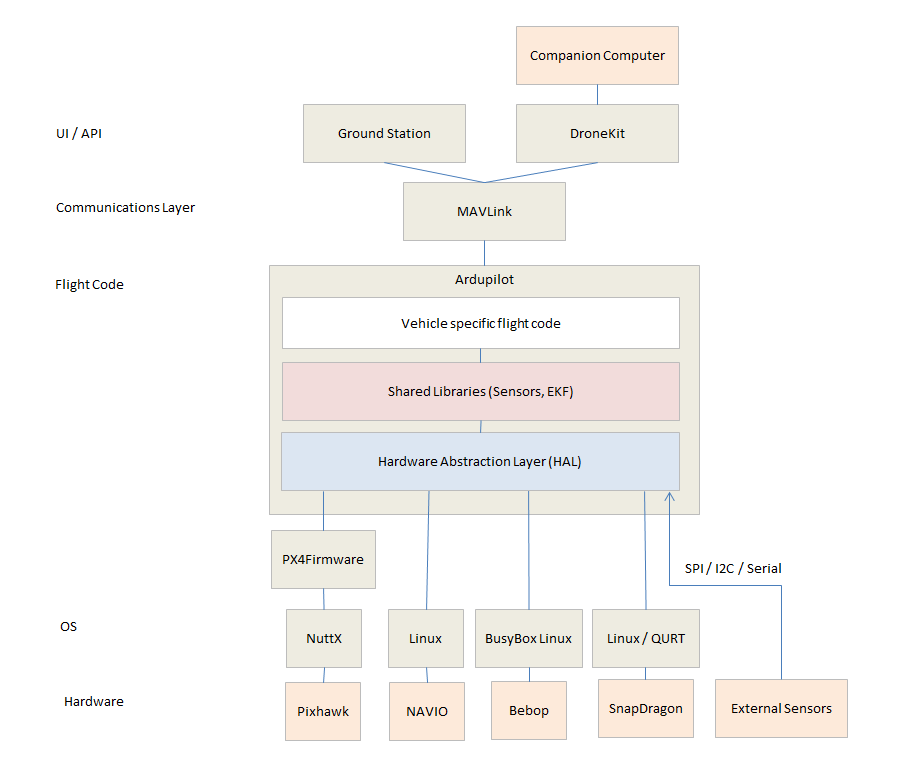
\includegraphics[scale=0.5]{images/ArduPilot_HighLevelArchecture.png}
    		\caption{Kiến trúc của Ardupilot}
    	\end{center}
    \end{figure}

			Cấu trúc cơ bản của ArduPilot gồm 5 phần chính:
			\begin{itemize}
    	\item Mã lập trình phương tiện (Vehicle code)
    	\item Các thư viện được chia sẻ (Shared libraries)
    	\item Lớp trừu tượng phần cứng (Hardware abstraction layer)
    	\item Các công cụ (Tool directories)
    	\item Các mã lập trình hỗ trợ ngoài (External support code: MAVLink, DroneKit)
    		\end{itemize}
    		
    		Như vậy nhóm sẽ tập trung vào phần lập trình quadcopter là mã nguồn ArduCopter. Cụ thể là viết phần chế độ bay theo bầy đàn ở lớp \textit{Mode} và file mã nguồn chế độ bay là \textit{Mode.cpp}.
    		
    \begin{figure}[h!]
    	\begin{center}
    		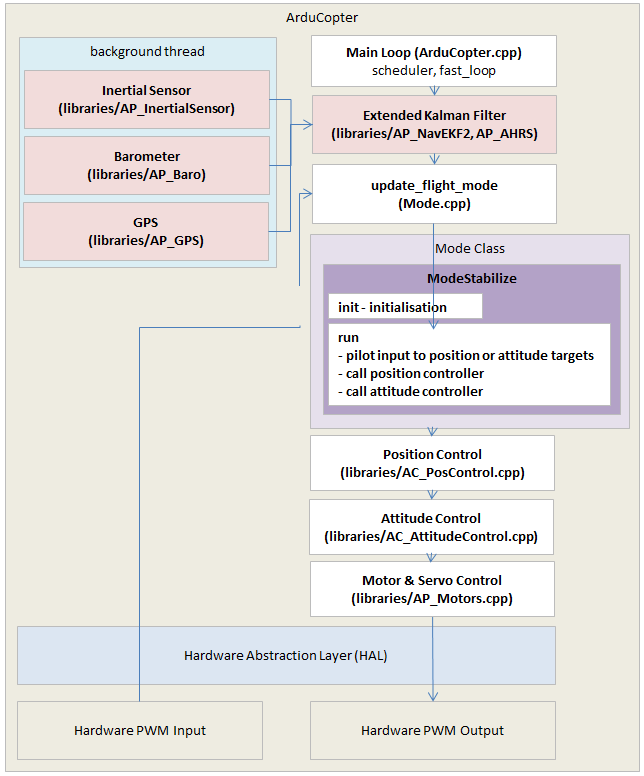
\includegraphics[scale=0.6]{images/copter-architecture.png}
    		\caption{Kiến trúc mã nguồn ArduCopter}
    	\end{center}
    \end{figure}
    
    \subsection{SITL Simulator}
    		Ardupilot cung cấp công cụ mô phỏng bay SITL (Software in the loop) cho phép mô phỏng bất kì phương tiện nào mà không cần đến phần cứng. Nó là một bản build từ mã nguồn Ardupilot chính nhưng cung cấp các thông tin phần cứng ảo. Lợi ích lớn nhất của SITL là cho phép sử dụng toàn bộ các công cụ phát triển bằng ngôn ngữ C++ trên máy tính như các trình gỡ rối, công cụ phân tích dữ liệu hay mô phỏng không gian ba chiều giúp khả năng phát triển và kiểm thử tính năng mới trên ArduPilot trở nên đơn giản hơn. 
    		
    \begin{figure}[h!]
    	\begin{center}
    		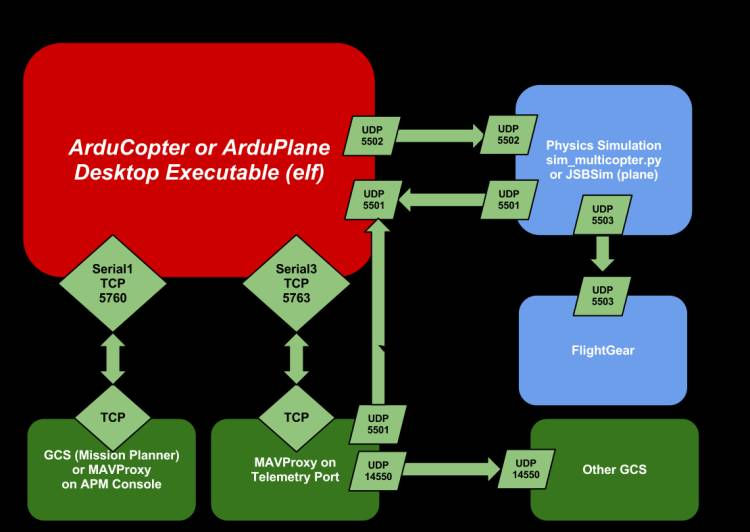
\includegraphics[scale=0.35]{images/ArdupilotSoftwareintheLoopSITL.jpg}
    		\caption{Kiến trúc phần mềm mô phỏng SITL}
    	\end{center}
    \end{figure}
    
    \begin{figure}[h!]
    	\begin{center}
    		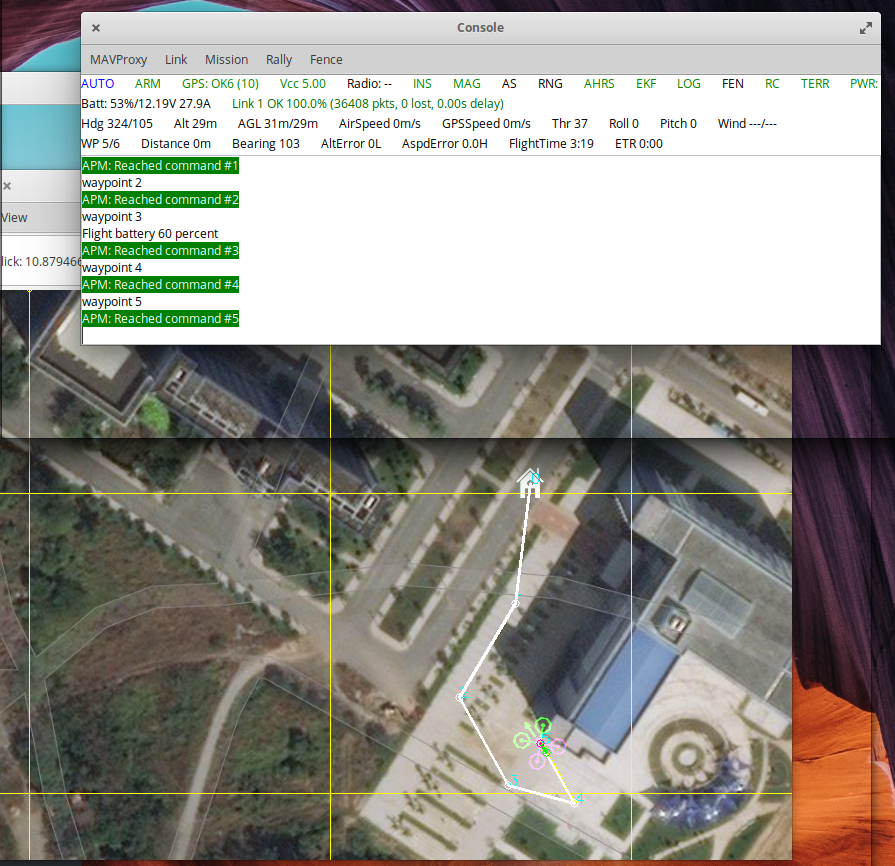
\includegraphics[scale=0.45]{images/simulating.png}
    		\caption{Mô phỏng một quadcopter bay theo quỹ đạo ở BKU cơ sở 2}
    	\end{center}
    \end{figure}
\chapter{Giai đoạn Luận văn tốt nghiệp}
    \section{Những công việc sẽ được thực hiện}
        \subsection{Hoàn thiện giải thuật bầy đàn}
        Nhóm chỉ mới đưa ra mô hình giải thuật bầy đàn chứ chưa có tiếp cận trên phương diện toán học để áp dụng vào lập trình. Trong giai đoạn luận văn nhóm sẽ hoàn thành giải thuật và áp dụng vào lập trình. 
        \subsection{Xây dựng phần cứng phù hợp và kết nối với chương trình điều khiển}
        Nhóm sẽ tiến hành hiện thực phần cứng dựa trên những gì đã tìm hiểu và kết nối với trình điều khiển Ardupilot bằng cách xây dựng bộ firmware phù hợp với phần cứng của nhóm thông qua lớp trừu tượng phần cứng (Hardware Abstraction Layer) trong Ardupilot.
        \subsection{Xây dựng chế độ bay theo bầy đàn trong Ardupilot}
        Dựa trên kiến trúc mã nguồn của Ardupilot mà nhóm đã tìm hiểu, nhóm sẽ sửa và viết thêm chế độ bay theo bầy đàn áp dụng giải thuật bầy đàn mà nhóm đã đưa ra.
    \section{Kế hoạch thực hiện}
        Mỗi thành viên của nhóm sẽ đảm nhiệm một nhiệm vụ chính nhưng đồng thời cũng hỗ trợ nhau cùng hoàn thành luận văn một cách hoàn chỉnh nhất. Nhiệm vụ cho mỗi thành viên như sau:
        \begin{itemize}
        \item Trần Lê Minh: đảm nhiệm việc tổ chức hoạt động nhóm, liên lạc với giảng viên, theo dõi tình hình và thúc đẩy tiến độ luận văn; hoàn thiện giải thuật bầy đàn và hỗ trợ nhóm trong việc xây dựng phần cứng và phần mềm; hoàn thiện báo cáo.
        \item Lê Huy Cường: xây dựng và hoàn thiện chế độ bay theo bầy đàn; hoàn thiện báo cáo; hỗ trợ xấy dựng phần cứng.
        \item Nguyễn Hoàng Thương: xây dựng và hoàn thiện phần cứng; hoàn thiện báo cáo; hỗ trợ xây dựng chế độ bay theo bầy đàn. 
    \end{itemize}
    Thời gian thực hiện luận văn là 15 tuần theo học kỳ chia làm ba giai đoạn:
    \begin{itemize}
        \item Giai đoạn 1 (5 tuần đầu): Tập trung vào xây dựng giải thuật bầy đàn và xây dựng chế độ bay theo bầy đàn, dùng công cụ mô phỏng bay để kiểm tra và tùy chỉnh.
        \item Giai đoạn 2 (5 tuần tiếp theo): Tập trung vào xây dựng và hoàn thiện phần cứng, áp dụng chế độ bay đã xây dựng vào thực tế để kiểm tra và điều chỉnh cho phù hợp.
        \item Giai đoạn 3 (5 tuần cuối): Tổng kết những kết quả thực hiện được, những khó khăn và đưa ra giải pháp, hoàn thiện báo cáo luận văn, chuẩn bị bài thuyết trình trước hội đồng.
    \end{itemize}
    	Nhóm sẽ sử dụng công cụ Slack trong liên lạc làm việc và Github để tổ chức mã nguồn báo cáo (Latex) cũng như mã nguồn chương trình.

\chapter{Kịch bản thử nghiệm} \label{chap:experiment}
    \section{Mục tiêu của thử nghiệm}
    \begin{itemize}
        \item Kiểm tra hoạt động của ứng dụng: node gateway thu thập dữ liệu từ các node cảm biến sau đó gửi lên cloud, ấn nút trên node gateway để điều khiển LED trên các node cảm biến.
        \item Chứng minh ứng dụng được hiện thực bằng giao thức mạng Mesh, cụ thể là vai trò của node relay.
        \item Chứng minh các node trong mạng có thể giao tiếp với nhau bằng cả 2 chiều gửi và nhận: node cảm biến gửi dữ liệu cho node gateway và nhận tín hiệu bật/tắt LED từ node gateway.
        \item Kiểm tra khoảng cách hoạt động tối đa giữa các node.
    \end{itemize}
    \section{Quá trình thử nghiệm}
        Nhóm thử nghiệm với 3 board phát triển, một board là node gateway còn lại là node cảm biến lần lượt gọi là node 0 và node 1. Đầu tiên cần tiến hành provision cho 2 node cảm biến: chỉ cần bật nguồn node gateway trước, rồi lần lượt bật nguồn node 0 và node 1. Sau đó tiến hành thử nghiệm bằng các kịch bản sau:
        \subsection{Kịch bản I: Thử nghiệm giao tiếp}
        \begin{itemize}
            \item Đặt 2 node 0 và node 1 ở gần node gateway, sau đó thử ấn nút gửi tín hiệu điều khiển LED thì thấy LED trên cả 2 node cảm biến chớp tắt.
            \begin{figure}[h!]
	    	 \begin{center}
	    		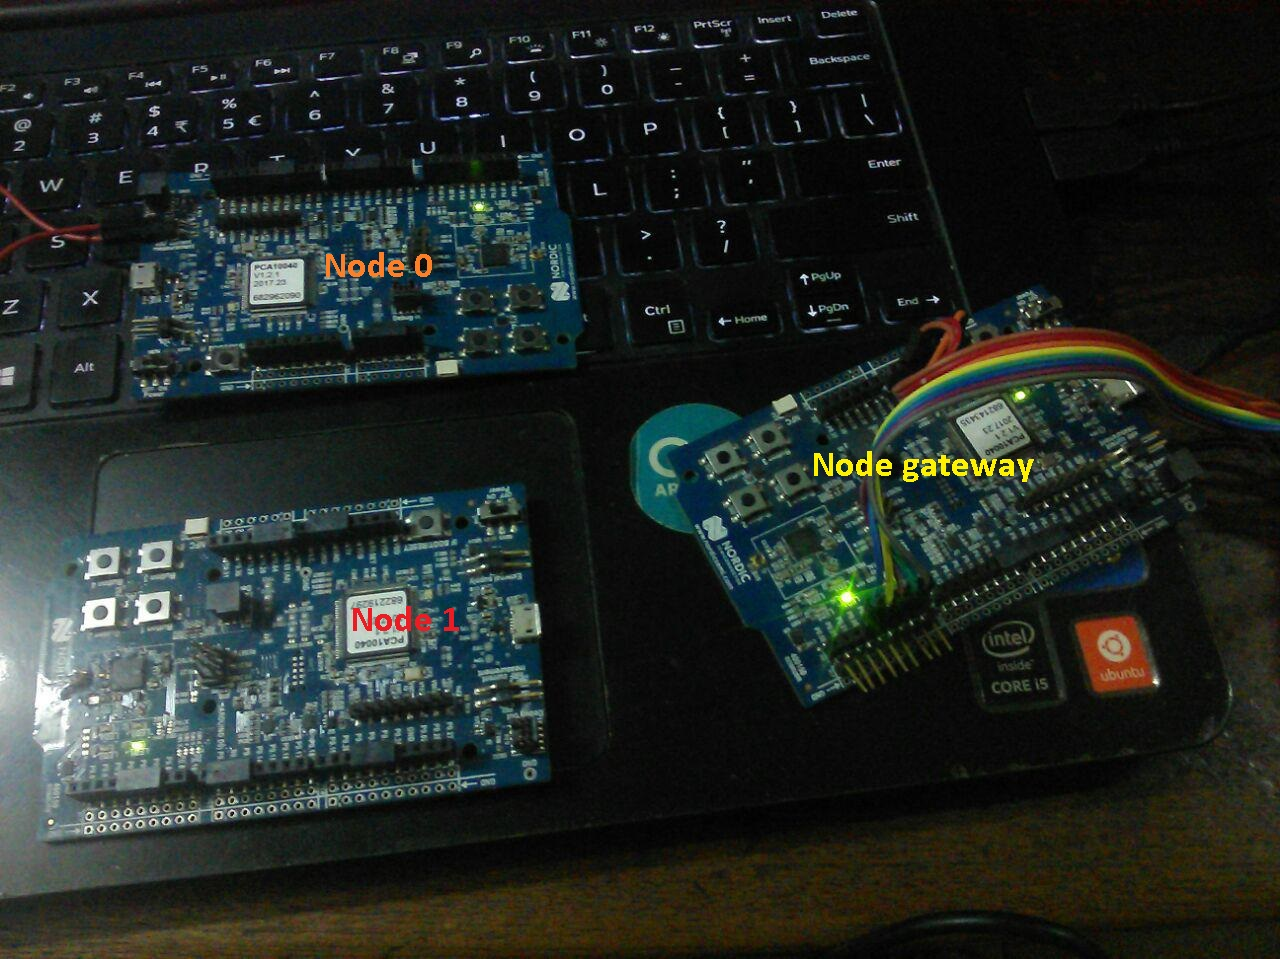
\includegraphics[scale=0.4]{images/ex1-1.jpg}
	    		\caption{Hình ảnh thử nghiệm I trong thực tế}
	    	\end{center}
    	\end{figure}
            \item Sau đó thử kích hoạt chế độ đọc và gửi dữ liệu cảm biến thì thấy node gateway nhận được dữ liệu và gửi lên server thành công. Có thể thử thay đổi dữ liệu bằng cách tăng nhiệt độ ở khu vực gần SoC nRF52832 trên Kit phát triển.
            \begin{figure}[h!]
	    	 \begin{center}
	    		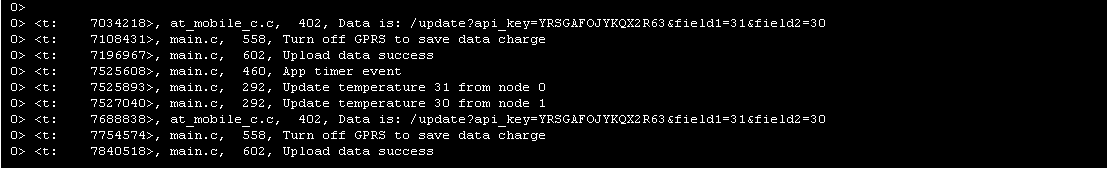
\includegraphics[scale=0.4]{images/ex1-2.png}
	    		\caption{Hình ảnh note gateway nhận được dữ liệu từ node cảm biến}
	    	\end{center}
    	\end{figure}
    	\begin{figure}[h!]
	    	 \begin{center}
	    		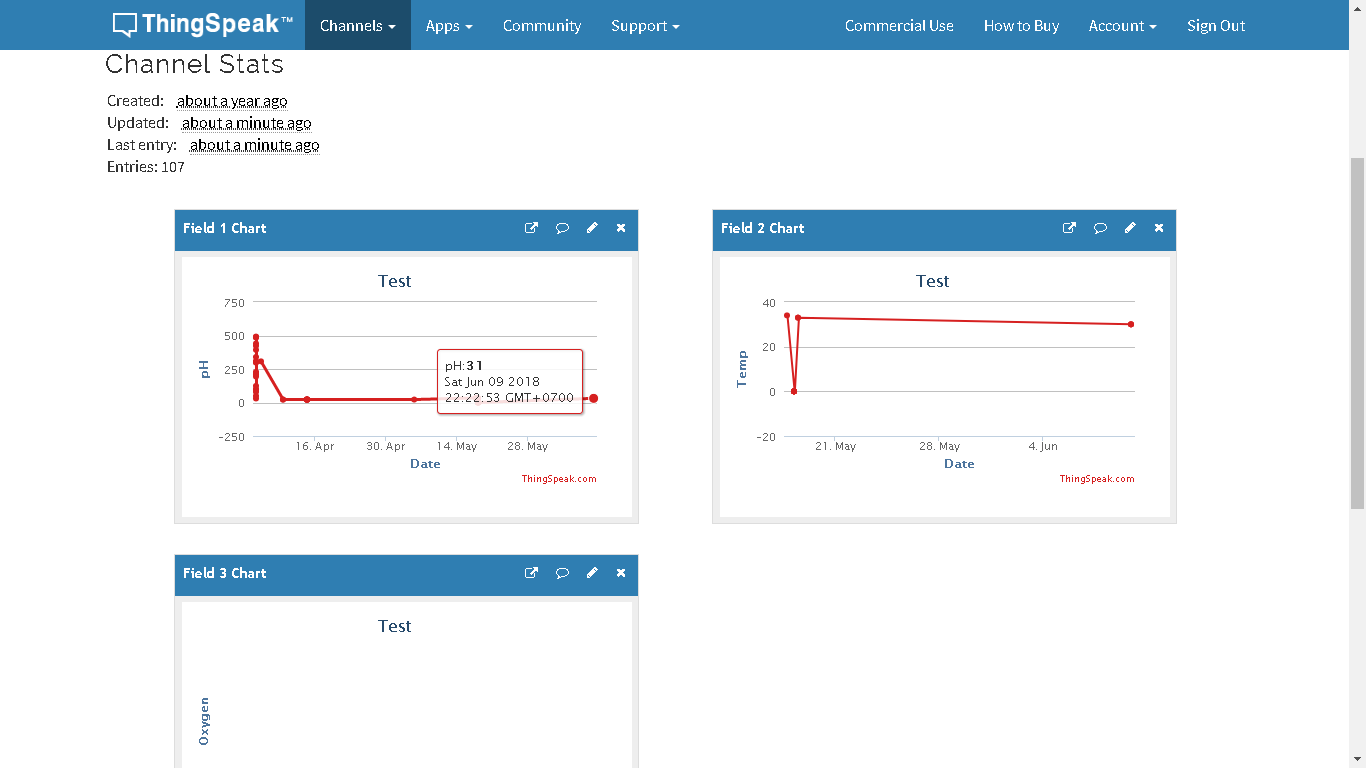
\includegraphics[scale=0.4]{images/ex1-3.png}
	    		\caption{Hình ảnh dữ liệu được cập nhật lên cloud}
	    	\end{center}
    	\end{figure}
            \item Thử tắt nguồn node 0 thì thấy node gateway báo lỗi không đọc được dữ liệu từ node 0, khi bật nguồn lại thì hoạt động bình thường trở lại.
        \end{itemize}
        \textbf{Kết quả thử nghiệm của kịch bản I chứng minh khả năng hoạt động của ứng dụng khi không có lỗi phát sinh.}
        \subsection{Kịch bản II: Thử nghiệm khoảng cách}
        \begin{itemize}
            \item Tiến hành với một node gateway và một node cảm biến là node 0, node gateway sẽ gửi lệnh điều khiển LED liên tục bằng cách nhấn nút.
            \item Sau đó dời node cảm biến dần dần ra xa cho đến khi LED trên node cảm biến không còn chớp tắt nữa thì dừng lại.
            \begin{figure}[h!]
	    	 \begin{center}
	    		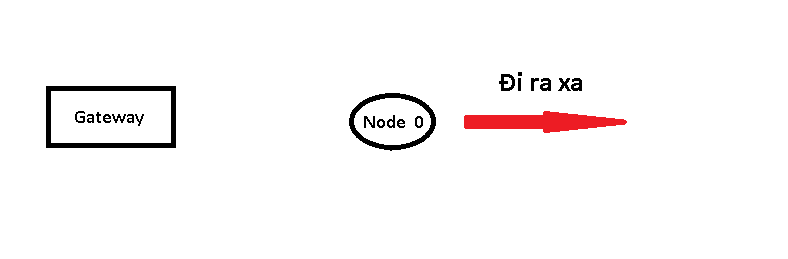
\includegraphics[scale=0.8]{images/ex2-1.png}
	    		\caption{Hình ảnh thử nghiệm II trong thực tế}
	    	\end{center}
        	 \end{figure}
            \item Khoảng cách giữa node gateway và node 0 lúc này là khoảng cách tối đa giữa 2 node của Bluetooth Mesh. Sau đó dời node 0 ra xa thêm khoảng 2m để tiến hành thử kịch bản III.
        \end{itemize}
        \textbf{Kết quả thử nghiệm của kịch bản II chứng tỏ khoảng cách giao tiếp tối đa giữa 2 node trong thực tế (không có vật cản) là khoảng từ 8-10m.}
        \subsection{Kịch bản III: Thử nghiệm truyền dữ liệu trong mạng mesh}
        \begin{figure}[h!]
	    	 \begin{center}
	    		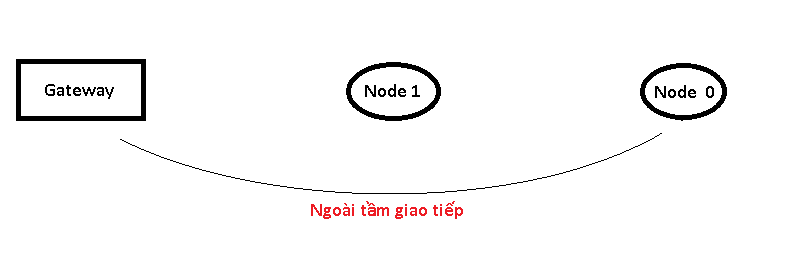
\includegraphics[scale=0.8]{images/ex3-1.png}
	    		\caption{Hình ảnh thử nghiệm III}
	    	\end{center}
        \end{figure}
        \begin{itemize}
            
            \item Sau khi node 0 đã nằm ngoại phạm vi giao tiếp với node gateway, đặt node 1 vào khoảng giữa 2 node này.
            \begin{figure}[h!]
	    	 \begin{center}
	    		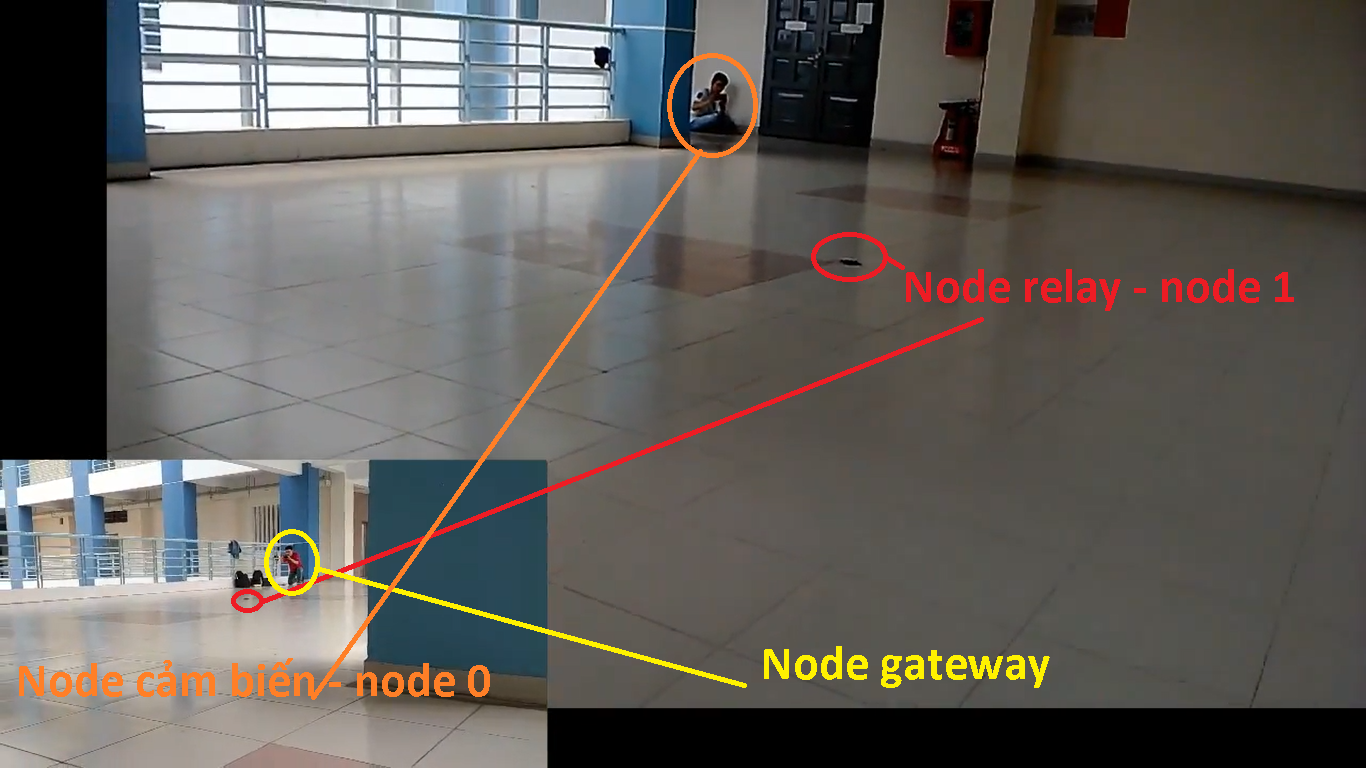
\includegraphics[scale=0.3]{images/ex3-2.png}
	    		\caption{Hình ảnh thử nghiệm III trong thực tế}
	    	\end{center}
    	\end{figure}
    	\newpage
            \item Sau đó tiến hành gửi tín hiệu điều khiển LED bằng node gateway, lúc này LED trên cả node 0 lẫn node 1 đều chớp tắt, chứng tỏ tín hiệu đã được node 1 relay lại và node 0 đã nhận được tín hiệu điều khiển (tín hiệu này gửi multicast nên cả 2 node 0 và 1 đều chớp LED).
            \begin{figure}[h!]
	    	 \begin{center}
	    		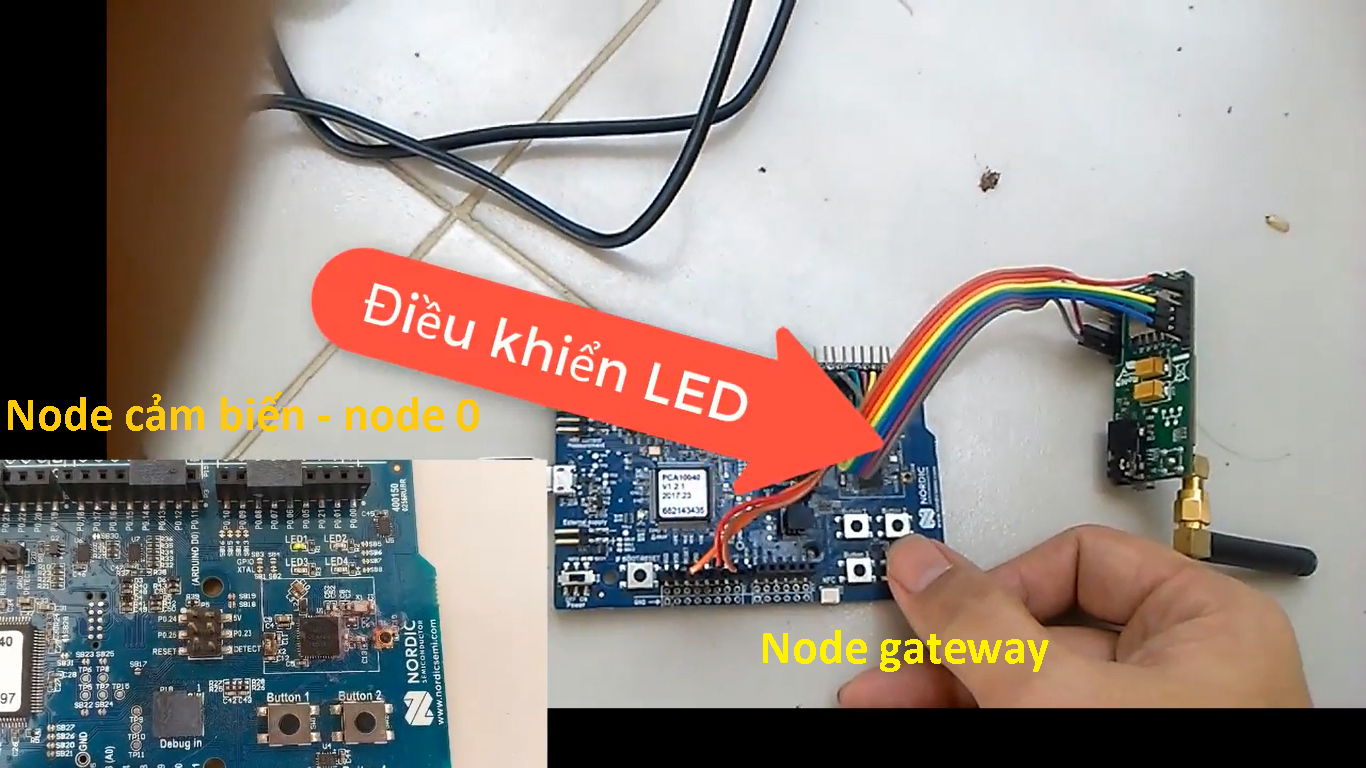
\includegraphics[scale=0.3]{images/ex3-3.png}
	    		\caption{Hình ảnh điều khiển LED trong thực tế}
	    	\end{center}
    	\end{figure}
        \end{itemize}
        \textbf{Kết quả thử nghiệm của kịch bản III chứng tỏ rằng node 1 đã đóng vai trò relay, giúp chuyển tiếp dữ liệu từ node gateway đến cho node 0.}






\chapter{Kết luận}\label{chap:conclude}
    \section{Đánh giá kết quả}
    	\subsection{Thành quả đạt được}
    	
    \begin{itemize}
        \item Tổng kết thành quả của nhóm trong quá trình nghiên cứu lý thuyết về Bluetooth Mesh: nguyên nhân ra đời, tiềm năng cạnh tranh, sơ lược về các lớp trong kiến trúc, cách truyền nhận dữ liệu giữa các node trong mạng, cách quản lý việc kết nối/ngắt kết nối.
        \item Kết quả nghiên cứu có thể được dùng làm tài liệu tham khảo cho những ai muốn làm quen với Bluetooth Mesh, giúp tiết kiệm thời gian tiếp cận.
        \item Hiện thực thành công ứng dụng sử dụng giao thức Bluetooth Mesh để giao tiếp. Mặc dù ứng dụng chưa quá hoàn thiện để có thể đưa vào thực tế, tuy nhiên cũng chứng minh được dữ liệu có thể đi theo 2 chiều gửi và nhận.
    \end{itemize}
    
    \subsection{Một số hạn chế của ứng dụng thử nghiệm}
    \begin{itemize}
        \item Chưa hỗ trợ thiết lập các thông số một cách linh hoạt: chu kỳ đọc, chu kỳ gửi, thông số cloud,...
        \item Chưa hỗ trợ lấy thông tin thiết bị
        \item Chưa hỗ trợ xóa node khỏi mạng
        \item Chưa hỗ trợ cơ chế xác thực mạnh khi provisioning
    \end{itemize}
    \section{Hướng phát triển}
    Do không đủ nhân lực nên nhóm chưa hiện thực tốt ứng dụng thử nghiệm, tuy nhiên nhóm có đề xuất một số cải tiến để ứng dụng thử nghiệm có thể trở thành ứng dụng trong thực tế:
    
    \begin{itemize}
        \item Tăng khả năng bảo mật bằng cách tăng giảm thông số node cảm biến tối đa trong mạng thông qua node gateway. Ví dụ hiện đang có 2 node cảm biến trong mạng, thông số node tối đa là 2, node cảm biến tiếp theo muốn tham gia vào mạng phải chờ node gateway tăng thông số node tối đa lên mới tham gia được. Bước này giúp tránh việc có node cảm biến tình cờ có được key vào mạng liền vào mạng với ý định xấu.
        \item Hiện thực giao diện cho node gateway để dễ dàng tiến hành các thao tác cấu hình như: thiết lập chu kỳ đọc dữ liệu, chu kỳ gửi dữ liệu, địa chỉ remote server, số node cảm biến tối đa, xóa node cảm biến ra khỏi mạng,...
        \item Hiện thực giao diện người dùng lấy dữ liệu từ remote server.
        \item Hiện thức một giao thức giao tiếp giữa các node để tránh tình trạng nghẽn mạng, quy trình xử lý khi node gateway mất kết nối hoặc node cảm biến mất kết nối.
    \end{itemize}
    
    \subsection{Tiềm năng trong thực tế}
    \begin{itemize}
        \item Hệ thống đèn lớn: Yêu cầu chính của hệ thống này là một bộ điều khiển có thể điều khiển một nhóm (có thể là cùng một tầng hoặc cùng một phòng) hay toàn bộ đèn, Bluetooth Mesh cực kỳ thích hợp trong ứng dụng này. Chỉ với một node client điều khiển và hàng ngàn node server với tốc độ đáp ứng nhanh, chức năng điều khiển đơn giản chỉ là bật tắt - thậm chí trong tương lai model này còn hỗ trợ độ mạnh yếu của đèn - là hệ thống có thể hoạt động tốt.
        \item Hệ thống cảm biến lớn: Những hệ thống như dây chuyền sản xuất tự động trong công nghiệp đòi hỏi có rất nhiều cảm biến đặt rải rác ở nhiều khâu trên dây chuyền. Tất cả các cảm biến đó sẽ gửi toàn bộ thông tin về một node trung tâm, sau đó node trung tâm này sẽ gửi 1 loạt dữ liệu đó lên server hoặc lưu vào một loại database nào đó, vì số lượng cảm biến trong hệ thống rất nhiều nên nếu mỗi node mỗi gửi dữ liệu sẽ dẫn đến một cuộc "DoS" nhẹ!
        \item Hệ thống theo dõi trong nhà: Rất nhiều cảm biến GPS hiện nay tín hiệu không đủ mạnh để định vị trong nhà, đặc biệt là ở tầng thấp. Bluetooth Mesh có thể khắc phục điểm yếu đó và kết hợp tốt với GPS, chúng ta có thể dựa vào mức độ mạnh yếu của tín hiệu và áp dụng thêm các thuật toán để xác định vị trí cũng như độ cao cụ thể của người hay vật trong nhà với độ chính xác cao.
    \end{itemize}
%\include{main/experiment}
%\include{main/conclusion}


%%%%%%%%%%%%%%%%%%%%%%%%%%%%%%%%%%%%%%%%%%%%%%
%%%%% TAIL: Bibliography, Appendix, CV
%%%%%%%%%%%%%%%%%%%%%%%%%%%%%%%%%%%%%%%%%%%%%%
\appendix
\chapter{Một số Model chuẩn}\label{models}

\section{Foundation models}
Foundation models have been defined in the core specification. Two of them are mandatory for all mesh nodes.

\begin{itemize}
	\item Configuration Server (mandatory)
	\item Configuration Client
	\item Health Server (mandatory)
	\item Health Client
\end{itemize}

\section{Generic models}
\begin{itemize}
\item Generic OnOff Server, used to represent devices that do not fit any of the model descriptions defined but support the generic properties of On/Off
\item Generic Level Server, keeping the state of an element in a 16-bit signed integer
\item Generic Default Transition Time Server, used to represent a default transition time for a variety of devices
\item Generic Power OnOff Server \& Generic Power OnOff Setup Server, used to represent devices that do not fit any of the model descriptions but support the generic properties of On/Off
\item Generic Power Level Server \& Generic Power Level Setup Server, including a Generic Power Actual state, a Generic Power Last state, a Generic Power Default state and a Generic Power Range state
\item Generic Battery Server, representing a set of four values representing the state of a battery
\item Generic Location Server \& Generic Location Setup Server, representing location information of an element, either global (Lat/Lon) or local
\item Generic User/Admin/Manufacturer/Client Property Server, representing any value to be stored by an element
\item Generic OnOff Client \& Generic Level Client
\item Generic Default Transition Time Client
\item Generic Power OnOff Client \& Generic Power Level Client
\item Generic Battery Client
\item Generic Location Client
\item Generic Property Client
\end{itemize}

\section{Sensors}
\begin{itemize}
\item Sensor Server \& Sensor Setup Server, representing a sensor device. Sensor device may be configured to return a measured value periodically or on request; measurement period (cadence) may be configured to be fixed or to change, so that more important value range is being reported faster.
\item Sensor Client
\end{itemize}

\section{Time and scenes}
\begin{itemize}
\item Time Server \& Time Setup Server, allowing for time synchronization in mesh network
\item Scene Server \& Scene Setup Server, allowing for up to 65535 scenes to be configured and recalled when needed.
\item Scheduler Server \& Scheduler Setup Server
\item Time Client, Scene Client \& Scheduler Client
\end{itemize}

\section{Lighting}
\begin{itemize}
\item Light Lightness Server \& Light Lightness Setup Server, representing a dimmable light source
\item Light CTL Server, Light CTL Temperature Server \& Light CTL Setup Server, representing a CCT or "tunable white" light source
\item Light HSL Server, Light HSL Hue Server, Light HSL Saturation Server \& Light HSL Setup Server, representing a light source based on Hue, Saturation, Lightness color representation
\item Light xyL Server \& Light xyL Setup Server, representing a light source based on modified CIE xyY color space.
\item Light LC (Lightness Control) Server \& Light LC Setup Server, representing a light control device, able to control Light Lightness model using an occupancy sensor and ambient light sensor. It may be used for light control scenarios like Auto-On, Auto-Off and/or Daylight Harvesting.
\item Light Lightness Client, Light CTL Client, Light HSL Client, Light xyL Client \& Light LC Client
\end{itemize}

\chapter{Flowchart quá trình remote provisioning}\label{remoteprov}
    \begin{figure}[h!]
    	\begin{center}
    		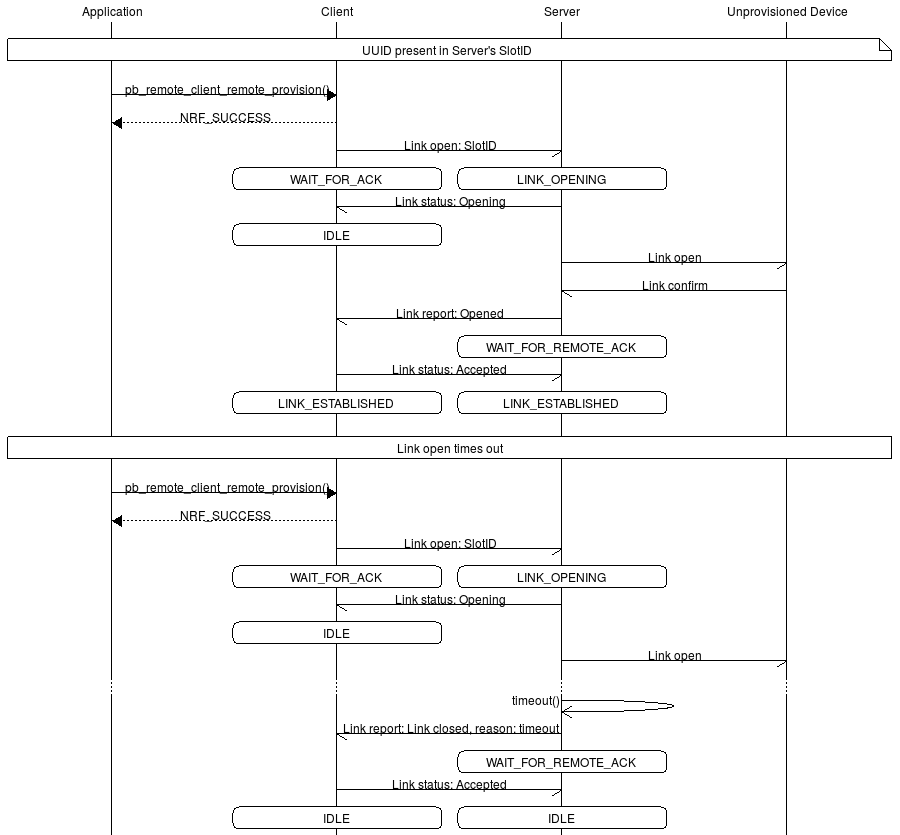
\includegraphics[scale=0.4]{images/msc_pb_remote_link_open.png}
    		\caption{Quá trình remote provisioning}
    	\end{center}
    \end{figure}
    
\chapter{Hướng dẫn thực thi ứng dụng}\label{guide}
\begin{enumerate}
\item Sau khi kết nối Kit PCA10040 với máy tính, sử dụng phần mềm nRFgo Studio để nạp Softdevice cho Kit.
            \begin{figure}[h!]
    	 \begin{center}
    		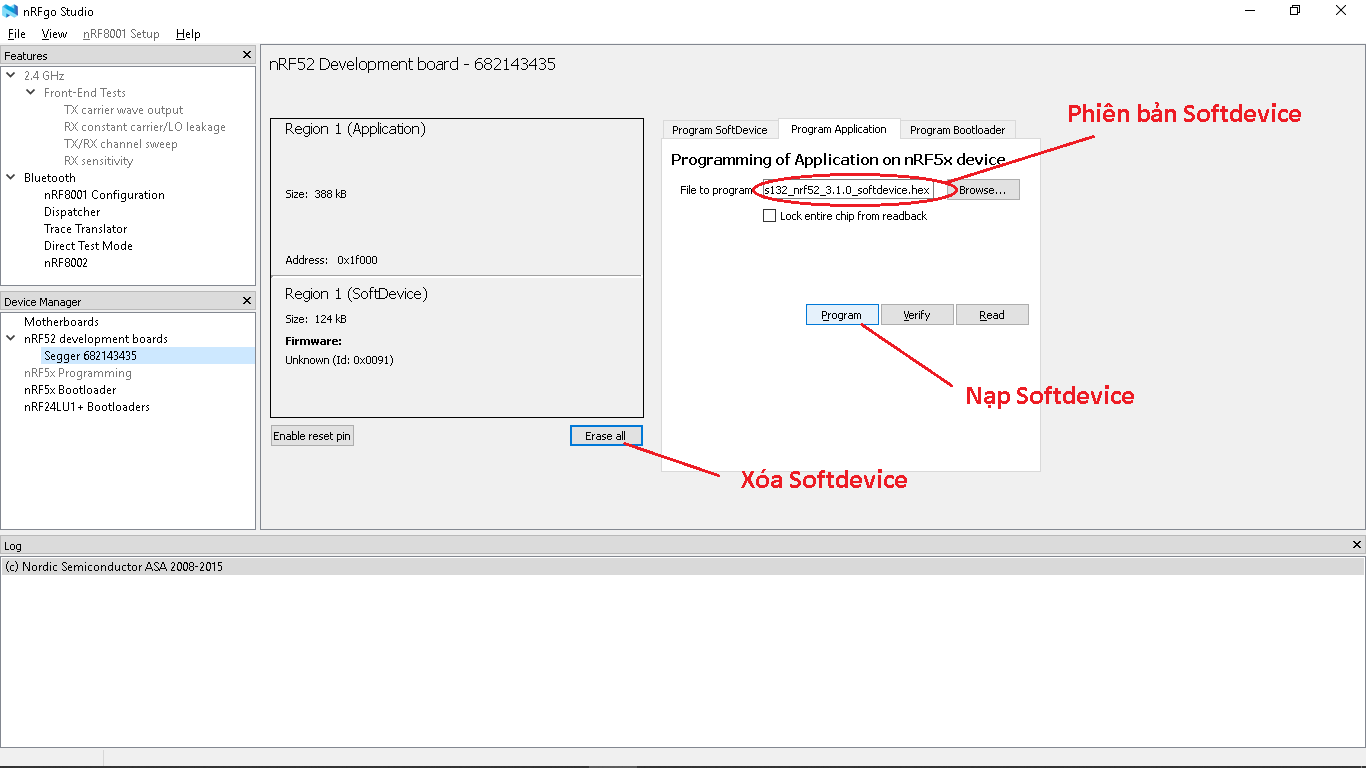
\includegraphics[scale=0.4]{images/app3-1.png}
    		\caption{Giao diện phần mềm nRFgo Studio}
    	\end{center}
    	\end{figure}
\item Sau khi đã nạp Softdevice, tiến hành nạp các chương trình khác nhau cho node cảm biến và node gateway. Node cảm biến sẽ dùng project - Embedded Studio Project - server còn node gateway sẽ dùng project client.
            \begin{figure}[h!]
    	 \begin{center}
    		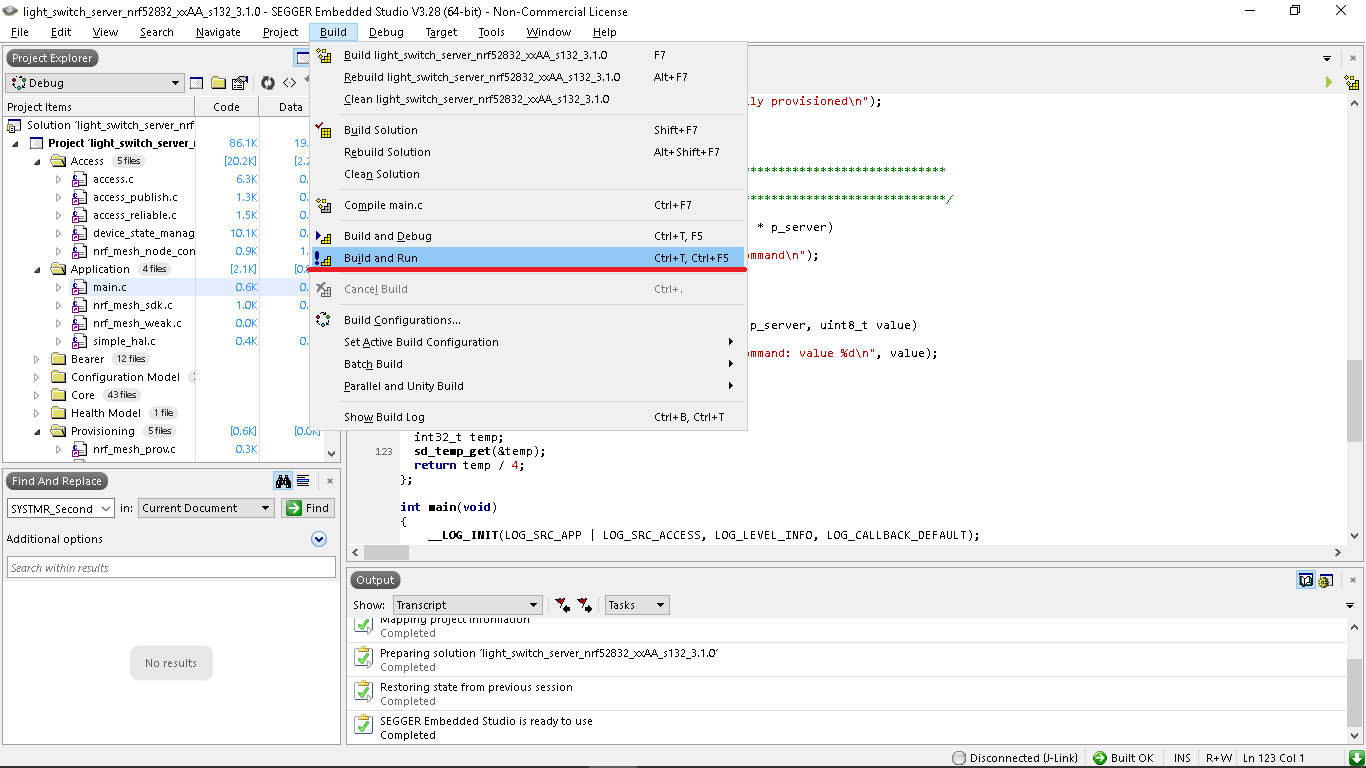
\includegraphics[scale=0.4]{images/app3-2.png}
    		\caption{Giao diện phần mềm Embedded Studio Project}
    	\end{center}
    	\end{figure}
    	\newpage
\item Để theo dõi quá trình thực thi của chương trình, sử dụng J-link RTT Viewer để xem quan sát quá trình.
	 \begin{figure}[h!]
    	 \begin{center}
    		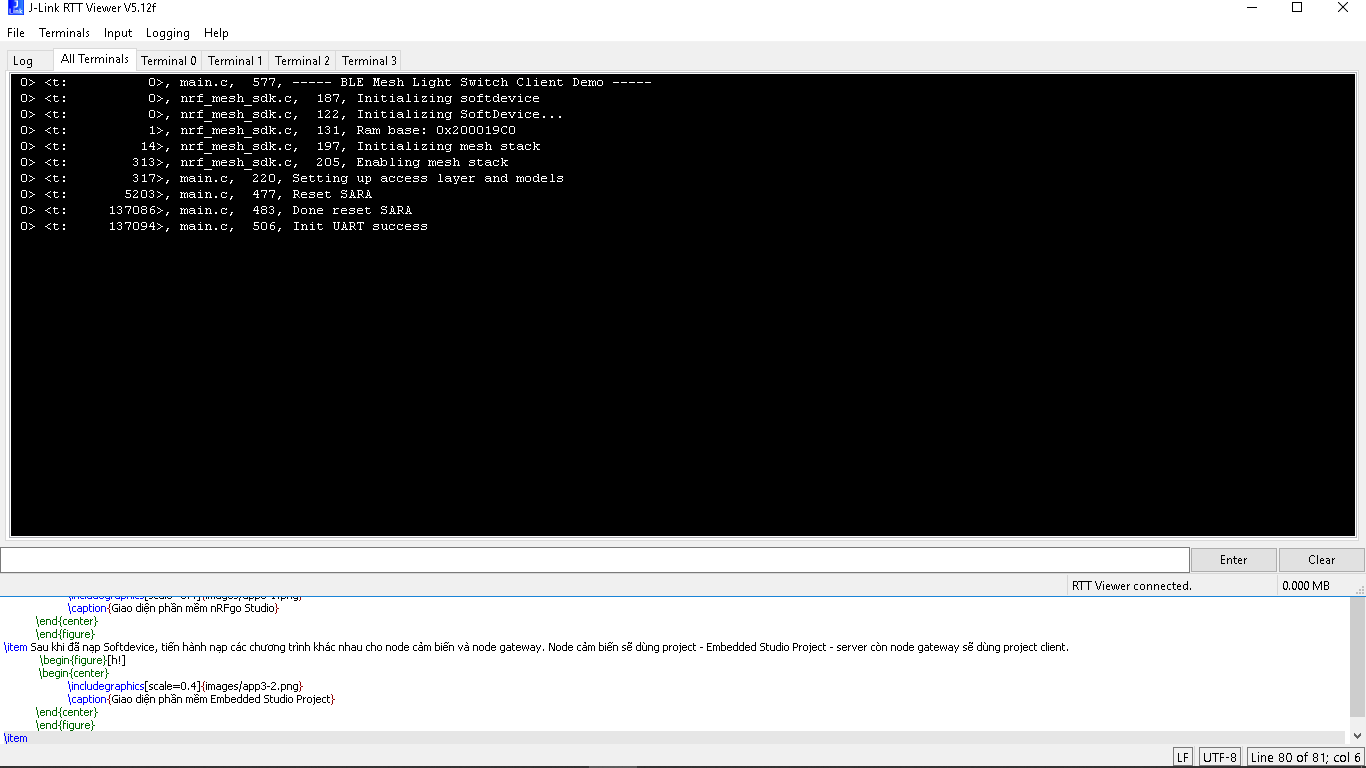
\includegraphics[scale=0.4]{images/app3-3.png}
    		\caption{Giao diện phần mềm J-link RTT Viewer}
    	\end{center}
    	\end{figure}
\end{enumerate}
\backmatter
\cleardoublepage
\renewcommand{\bibname}{Tài liệu tham khảo}
\begin{thebibliography}{80}

%[1]
\bibitem{arducopter}
Ardupilot Copter Introduction
\\\texttt{\url{http://ardupilot.org/copter/docs/introduction.html}}

%[2]
\bibitem{arducopterdev}
Ardupilot Development Site
\\\texttt{\url{http://ardupilot.org/dev/index.html}}

%[3]
\bibitem{caohoangtien}
Cao Hoàng Tiến, \textit{Điều khiển bám quỹ đạo cho mô hình máy bay bốn cánh quạt - Quadrotor}, 2014

\end{thebibliography}
\addcontentsline{toc}{chapter}{Tài liệu tham khảo}


% Add your glossary here
% Add your index here
% Photographic credits (list of pictures&images that have been used with names of the person holding the copyright for them)
%\include{tail/cv}

\end{document}
\grid
